\documentclass{sheftech}
\usepackage[T1]{fontenc}
\usepackage[latin9]{inputenc}
\setcounter{secnumdepth}{3}
\setcounter{tocdepth}{3}
\usepackage{url}
\usepackage{amsbsy}
\usepackage{amstext}
\usepackage{graphicx}
\usepackage[authoryear]{natbib}
\usepackage{a4wide}

\makeatletter


\@ifundefined{showcaptionsetup}{}{%
 \PassOptionsToPackage{caption=false}{subfig}}
\usepackage{subfig}
\makeatother

tabularnewlinebegin{document}
\title{The Gaussian Process Latent Variable Model}
\date{27th January 2006}
\author{Neil D. Lawrence}
\maketitle
\begin{abstract}
The Gaussian process latent variable model (GP-LVM) is a recently
proposed probabilistic approach to obtaining a reduced dimension representation
of a data set. In this tutorial we motivate and describe the GP-LVM,
giving reviews of the model itself and some of the concepts behind
it. 
\end{abstract}

\section{Introduction}

The Gaussian process latent variable model (GP-LVM) is a powerful
approach to probabilistic non-linear dimensionality reduction. It
was inspired by, and is related to, a class of probabilistic dimensionality
reduction techniques known as latent variable models.  In this tutorial
we will review in detail a \emph{linear} dimensionality reduction
technique known as probabilistic PCA \citep{Tipping:probpca99}. As
we shall see, by taking an alternative view point of the latent variable
model behind PCA we can develop a novel, alternative, interpretation
of probabilistic PCA. One that, as it turns out, will lend itself
to an elegant non-linearisation through Gaussian processes. However
before discussing the resulting model in detail we will conduct a
brief review of Gaussian processes, discussing what it means to have
a prior over functions and what Gaussian distributed functions can
look like. 

Finally we shall round off by discussing the characteristics of the
GP-LVM  and by mentioning some extensions of the model.

In the notes we will make use of examples that can be recreated through
code downloaded from \url{https://inverseprobability.com/GPmat}.
An additional package of demonstrations associated with this presentation
has been placed at \url{https://inverseprobability.com/oxford}.

\section{Motivation}

Many data sets we deal with are high dimensional. The `curse of dimensionality'
implies that to correctly understand the structure of a high dimensional
data set we need many data points, exponentially many in the number
of dimensions. However, in practice we find that we often do very
well with much smaller data sets than we might expect to need. One
possible reason for this is that many data sets of interest, while
seemingly high dimensional, have an intrinsic dimensionality which
is much lower. Let us consider the example of handwritten digits.

In Figure~\ref{cap:digit6} we show a hand-written 6 taken from the
USPS Cedar CD-ROM handwritten digits training set.
\begin{figure}
\begin{centering}
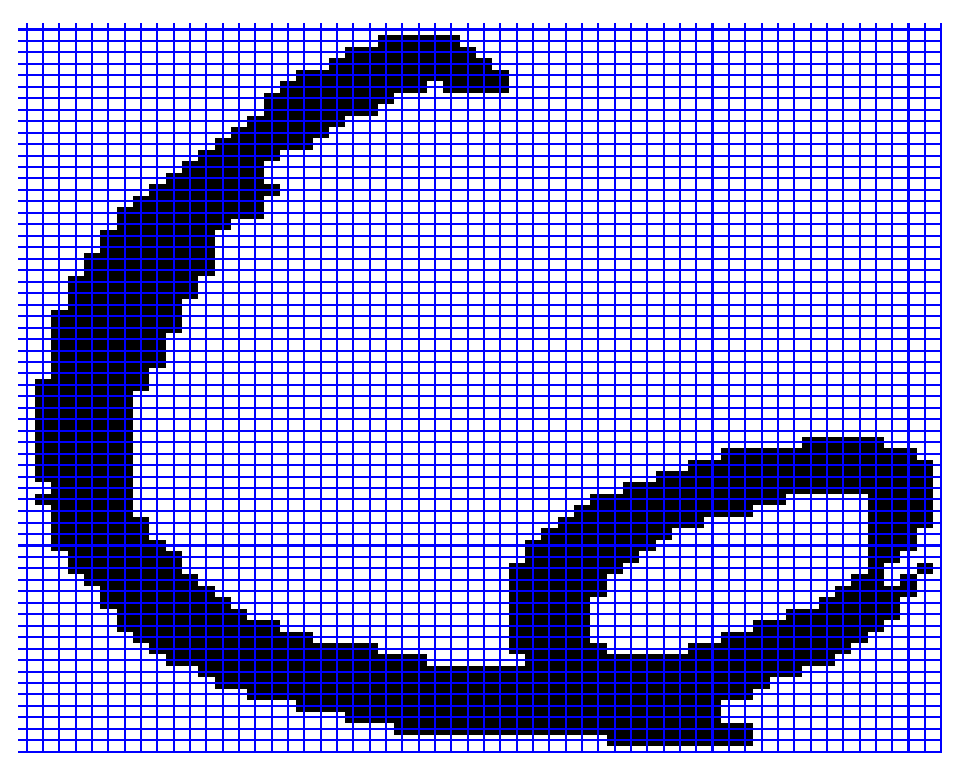
\includegraphics[width=0.5\textwidth]{diagrams/digitSix}
\par\end{centering}
\small 

\caption{Digit 6 from the USPS Cedar CD-ROM. The digit is 64 pixels by 57 pixels
giving it 3,648 dimensions. \label{cap:digit6}}
\end{figure}
The data point is 3,648 dimensional as it is printed in a 64 pixel
by 57 pixel image. However, if our data is based on a few simple transformations
of this digit, it may not span all 3,648 dimensions of the space.
To see this consider Figure~\ref{cap:twoManifolds}. Here we have
created a data set by rotating the original digit 360 times, each
time by one degree. The data is then projected onto its second and
third principal components. The resulting projection clearly shows
a circular shape. There is some noise (presumably associated with
the nearest neighbour interpolation used in the rotation of the image)
but the structure of the space is clear. Further examination of the
principal components (which is possible with the software on line)
also reveals that the dataset is inherently one dimensional. 

\begin{figure}
\begin{centering}
\subfloat[]{

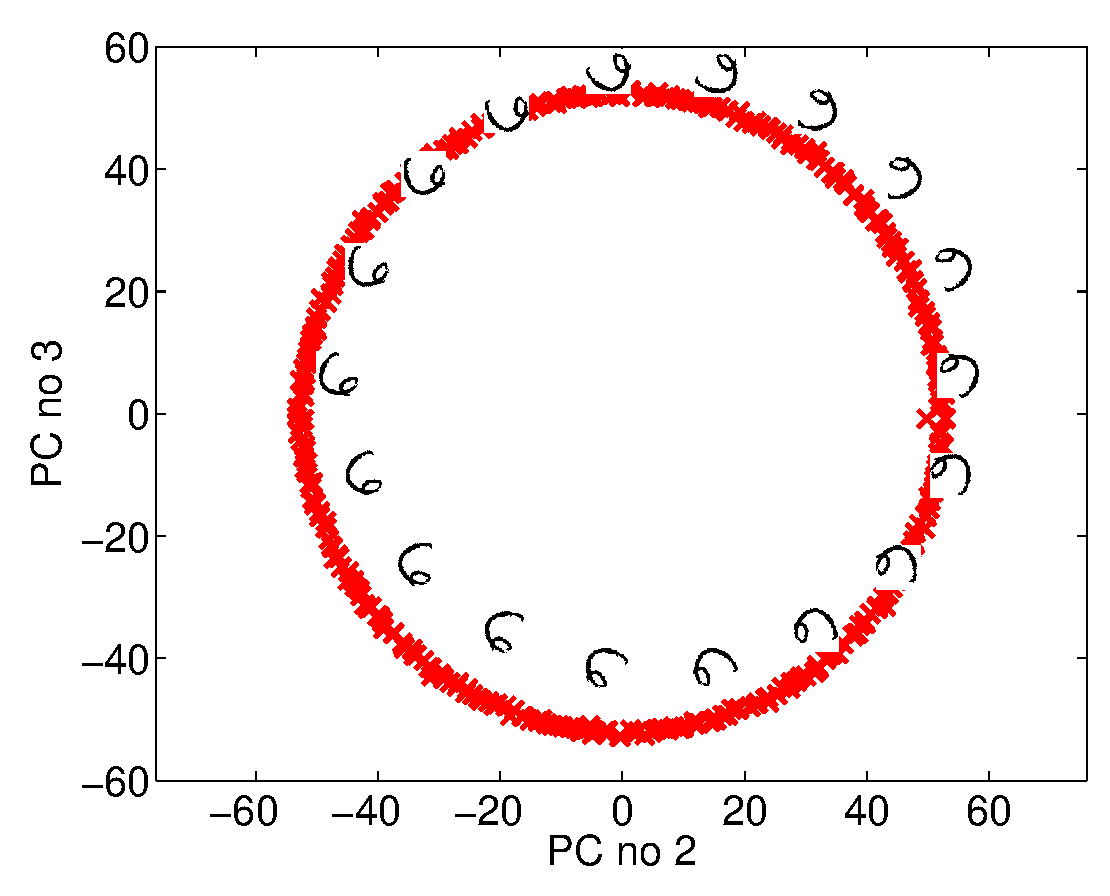
\includegraphics[width=0.45\textwidth]{diagrams/demManifoldPrint1}}\hfill{}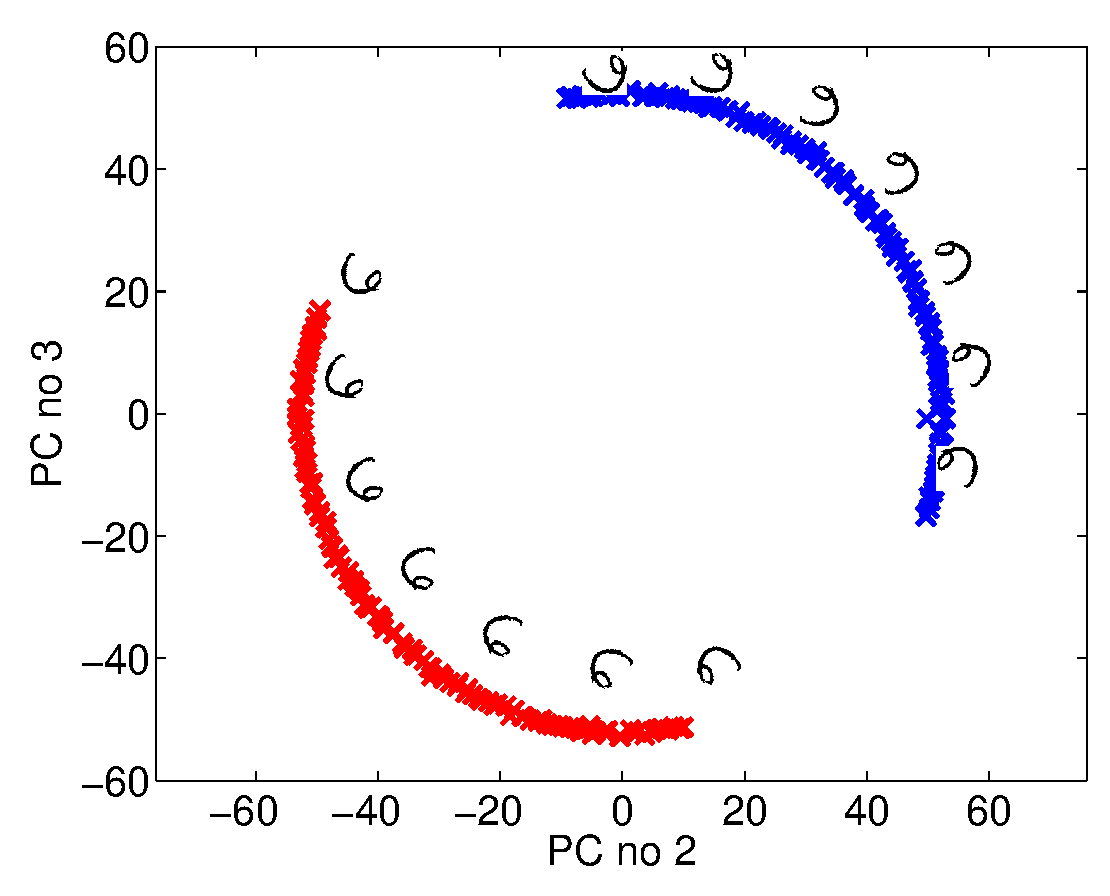
\includegraphics[width=0.45\textwidth]{diagrams/demManifoldPrint2}
\par\end{centering}
\caption{Rotation of handwritten 6. A data set is generated by rotating the
original image 360 times (\texttt{prepDemManifold}). The data set
is then visualised by projecting into the second and third principal
component. In (a) the full rotation is visualised (\texttt{demManifoldPrint({[}2
3{]}, 'all')}), in (b) some rotations are assumed to be associated
with the digit 6 and others from the digit 9 (\texttt{demManifoldPrint({[}2
3{]}, 'sixnine')}).\label{cap:twoManifolds}}
\end{figure}

In practice of course real data sets will not be generated by a simple
rotation of a one dimensional space. However, it seems reasonable
to assume that a data set might consist of a fixed number of `prototypes'
which undergo a limited number of transformations and then are, perhaps,
corrupted by some noise. If this is the case, then it makes sense
to model high dimensional data by seeking a low dimensional representation.
In statistics the standard approach to this problem is multi-dimensional
scaling (MDS, see \emph{e.g.} \citet{Mardia:multivariate79}). More
recently in machine learning several spectral approaches have been
proposed \citep{Tenenbaum:isomap00,Roweis:lle00,Weinberger:learning04}
some of which may be seen as classical MDS with a particular approach
to learning a distance matrix. We wish to focus on probabilistically
inspired approaches. Having an algorithm with a probabilistic interpretation
allows the algorithm to be extended in a logical manner and eases
integration of the approach in a larger system. All currently published
extensions and applications of the GP-LVM take advantage of its probabilistic
interpretation in one form or another \citep{Grochow:styleik04,Urtasun:priors05,Wang:gpdm05,Shon:learning05}.

In the next section we discuss, perhaps, the simplest latent variable
model that can be used for dimensional reduction, probabilistic PCA.
The model is fundamentally linear, but it illustrates the basic concepts
behind latent variable models.  We will then briefly review Gaussian
processes (in Section~\ref{sec:GPs}) after which we will introduce
the fundamental re-thinking of the latent variable model behind PCA
that enables dual probabilistic PCA and leads to the GP-LVM (Section~\ref{sec:GPLVM}).
We will then show various results achieved with the GP-LVM and briefly
mention some enhancements.

\section{Probabilistic PCA\label{sec:PPCA}}

Probabilistic PCA is a simple latent variable model where the latent
space, $\mathbf{X}=\left[\mathbf{x}_{1},\dots,\mathbf{x}_{N}\right]^{\textrm{T}}$
is assumed to be related to the \emph{centred data set}, $\mathbf{Y}=\left[\mathbf{y}_{1},\dots,\mathbf{y}_{N}\right]^{\textrm{T}}$
through a linear mapping that is corrupted by noise, 
\[
\mathbf{y}_{n}=\mathbf{W}\mathbf{x}_{n}+\boldsymbol{\eta}_{n},
\]
where the mapping is given by $\mathbf{W}\in\Re^{D\times q}$ with
$D$ the dimension of the data space and $q$ the dimension of the
latent space and $\boldsymbol{\eta}_{n}$ is a vector of noise terms.
For the particular case of probabilistic PCA, the noise is taken to
be Gaussian distributed,
\[
p\left(\boldsymbol{\eta}_{n}|\beta\right)=N\left(\boldsymbol{\eta}_{n}|\mathbf{0},\beta^{-1}\mathbf{I}\right),
\]
with a mean of zero and a spherical covariance given by $\beta^{-1}\mathbf{I}$.
The parameter $\beta$ is an inverse variance and is therefore referred
to as a precision.

The conditional probability of the data given the latent space can
be written as
\[
p\left(\mathbf{y}_{n}|\mathbf{x}_{n},\mathbf{W},\beta\right)=N\left(\mathbf{y}_{n}|\mathbf{W}\mathbf{x}_{n},\beta^{-1}\mathbf{I}\right),
\]
and assuming independence across data points we have
\begin{equation}
p\left(\mathbf{Y}|\mathbf{X},\mathbf{W},\beta\right)=\prod_{n=1}^{N}N\left(\mathbf{y}_{n}|\mathbf{W}\mathbf{x}_{n},\beta^{-1}\mathbf{I}\right).\label{eq:ppcaLikelihood}
\end{equation}
Following the Bayesian nomenclature, in anticipation of a prior distribution
over the latent space, this term can be seen as the \emph{likelihood}
of the data $\mathbf{Y}$ given $\mathbf{X}$. We note in passing
that it is also the likelihood associated with a least-squares multi-variate
regression: if we are given $\mathbf{X}$ and maximise the likelihood
with respect to $\mathbf{W}$ we recover
\[
\hat{\mathbf{W}}\mathbf{X}^{\textrm{T}}\mathbf{X}=\mathbf{Y}^{\textrm{T}}\mathbf{X},
\]
which may be solved for $\hat{\mathbf{W}}$ to obtain the least squares
regression estimate of $\mathbf{W}$. In probabilistic PCA however,
the values of $\mathbf{X}$ aren't given, they are \emph{nuisance
parameters}. The standard approach when dealing with these parameters
is to consider a \emph{prior distribution} over the latent space,
$p\left(\mathbf{X}\right)$, and seek to marginalise the values of
$\mathbf{X}$. 

\subsection{Gaussian Prior}

The choice of prior distribution will clearly have an effect on the
optimum value of $\mathbf{W}$. If the latent distributions are chosen
to be independent across $q$ and non-Gaussian, the latent variable
model behind independent component analysis \citep{Bell:ica95,MacKay:ica96}
is recovered in the limit as $\beta\rightarrow\infty$. It has also
long been known that if the latent distribution is chosen to be Gaussian
then PCA is recovered in the limit as $\beta\rightarrow\infty$ (this
observation inspired sensible PCA \citep{Roweis:SPCA97}). More interestingly
\citet{Tipping:probpca99} showed that if the latent distribution
is taken to be Gaussian then the maximum likelihood solution for $\mathbf{W}$
can span the principal subspace of the data even when $\beta$ is
finite. The form of the Gaussian prior is chosen by convention\footnote{Using non-zero mean and non-unit covariance merely leads to a redundant
parameterisation of the model. However this redundant parameterisation
can be exploited in certain circumstances to give faster converging
algorithms \citep{Sanguinetti:accounting05}.} to be zero mean and unit covariance,
\begin{equation}
p\left(\mathbf{X}\right)=\prod_{n=1}^{N}p\left(\mathbf{x}_{n}\right)=\prod_{n=1}^{N}N\left(\mathbf{x}_{n}|\mathbf{0},\mathbf{I}\right).\label{eq:ppcaPrior}
\end{equation}
The marginal likelihood can then be computed as follows
\begin{eqnarray}
p\left(\mathbf{Y}|\mathbf{W},\beta\right) & = & \prod_{n=1}^{N}\int N\left(\mathbf{y}_{n}|\mathbf{W}\mathbf{x}_{n},\beta^{-1}\mathbf{I}\right)N\left(\mathbf{x}_{n}|\mathbf{0},\mathbf{I}\right)d\mathbf{x}_{n}\label{eq:firstLine}\\
 & \propto & \prod_{n=1}^{N}\int\exp\left(-\frac{1}{2}\left(\beta\mathbf{y}_{n}^{\textrm{T}}\mathbf{y}_{n}-2\beta\mathbf{y}_{n}^{\textrm{T}}\mathbf{W}\mathbf{x}_{n}+\mathbf{x}_{n}^{\textrm{T}}\left(\beta\mathbf{W}^{\textrm{T}}\mathbf{W}+\mathbf{I}\right)\mathbf{x}_{n}\right)\right)d\mathbf{x}_{n}\label{eq:secondLine}\\
 & \propto & \prod_{n=1}^{N}\exp\left(-\frac{1}{2}\left(\mathbf{y}_{n}^{\textrm{T}}\left(\beta\mathbf{I}-\beta^{2}\mathbf{W}\left(\beta\mathbf{W}^{\textrm{T}}\mathbf{W}+\mathbf{I}\right)^{-1}\mathbf{W}^{\textrm{T}}\right)\mathbf{y}_{n}\right)\right)\label{eq:thirdLine}
\end{eqnarray}
where the first line (\ref{eq:firstLine}) is obtained through multiplying
(\ref{eq:ppcaLikelihood}) and (\ref{eq:ppcaPrior}) to obtain the
joint likelihood, and introducing the intergrad to marginalise $\mathbf{X}$.
The second line (\ref{eq:secondLine}) is obtained by expanding the
squares, (\ref{eq:thirdLine}) is then obtained by standard integrals
on Gaussians (see Appendix B on Gaussian integrals in \citet{Bishop:book95}
for a proof). We can obtain the final solution through inspection
of (\ref{eq:thirdLine}): the matrix associated with the quadratic
term has the form of the matrix inversion lemma\footnote{In its most general form the matrix inversion lemma is $\left(\mathbf{A}+\mathbf{BC}\mathbf{D}\right)^{-1}=\mathbf{A}^{-1}-\mathbf{A}^{-1}\mathbf{B}\left(\mathbf{C}^{-1}+\mathbf{D}\mathbf{A}^{-1}\mathbf{B}\right)^{-1}\mathbf{D}\mathbf{A}^{-1}$.}
and there are no linear terms in $\mathbf{y}_{n}$, implying that
the solution is a product of zero mean Gaussians,
\begin{equation}
p\left(\mathbf{Y}|\mathbf{W},\beta\right)=\prod_{n=1}^{N}N\left(\mathbf{y}_{n}|\mathbf{0},\mathbf{C}\right),\label{eq:ppcaMarginaLikelihood}
\end{equation}
where the covariance is given by $\mathbf{C}=\mathbf{WW}^{\textrm{T}}+\beta^{-1}\mathbf{I}$.
This is immediately recognised as a reduced rank representation of
the covariance. Since $\mathbf{W}\in\Re^{D\times q}$ the matrix $\mathbf{W}\mathbf{W}^{\textrm{T}}\in\Re^{D\times D}$
will have rank of at most $q$. For finite $\beta$ the term $\beta^{-1}\mathbf{I}$
then acts as a `regulariser' to ensure that the resulting covariance
has full rank and the distribution is thereby properly defined. 

This model was suggested simultaneously by \citet{Roweis:SPCA97,Tipping:probpca99},
but \citet{Tipping:probpca99} also provided the proof that the maximum
likelihood solution for $\mathbf{W}$ spans the principal sub-space
of the data. The proof for the dual probabilistic PCA we introduce
in Section~\ref{sec:GPLVM} closely tracks the proof of \citet{Tipping:probpca99}
so we omit the details here, merely giving the result. The optimum
value for $\mathbf{W}$ is given by 
\[
\hat{\mathbf{W}}=\mathbf{U}_{q}^{\prime}\mathbf{L}\mathbf{V}^{\textrm{T}}
\]
where $\mathbf{U}_{q}^{\prime}$ are the $q$ eigenvectors of the
covariance matrix $N^{-1}\mathbf{Y}^{\textrm{T}}\mathbf{Y}$ associated
with the $q$ largest eigenvalues, $\left\{ \lambda_{i}\right\} _{i=1}^{q}$
which may be obtained by solving
\begin{equation}
N^{-1}\mathbf{Y}^{\textrm{T}}\mathbf{YU}^{\prime}=\mathbf{U}^{\prime}\Lambda.\label{eq:ppcaEigenValueProblem}
\end{equation}
 The matrix $\mathbf{L}$ is diagonal and its $i$th diagonal element
is given by $l_{i}=\left(\lambda_{i}-\beta^{-1}\right)^{\frac{1}{2}}$. 

The principal components of a data set are the eigenvectors of the
covariance matrix, and the principal sub-space is the space spanned
by those eigenvectors. We therefore see that the solution for probabilistic
PCA spans the $q$-dimensional principal sub-space of the data. 

We will revisit probabilistic principal component analysis in Section~\ref{sec:GPLVM}
when we discuss the Gaussian process latent variable model. First
we will briefly review Gaussian processes.

\section{Gaussian Processes\label{sec:GPs}}

Gaussian processes \citep{Ohagan:curve78,Ohagan:numerical92,Williams:Gaussian96,Williams:prediction98,MacKay:gpintroduction98,Rasmussen:book06}
are probability distributions over functions. We can combine a Gaussian
process prior with a likelihood (or noise model) to obtain a posterior
over functions. If the likelihood is also Gaussian the form of the
posterior will also be a Gaussian process. In practice the likelihood
is often non-Gaussian but even in this case we typically approximate
the posterior process with a Gaussian process.

\subsection{A Prior Over Functions}

A distribution over functions is seemingly non-sensical as functions
are infinite dimensional objects. However, let us proceed by considering
a finite Gaussian distribution over some values instantiated from
a function $\mathbf{f}=\left\{ f_{n}\right\} _{n=1}^{N}\in\Re^{N\times1}$.
If we assume that these values are drawn from a Gaussian distribution
with mean zero and covariance $\mathbf{K}$, then we can write
\begin{eqnarray*}
p\left(\mathbf{f}|\mathbf{K}\right) & = & N\left(\mathbf{f}|\mathbf{0},\mathbf{K}\right)\\
 & = & \frac{1}{\left(2\pi\right)^{\frac{N}{2}}\left|\mathbf{K}\right|^{\frac{1}{2}}}\exp\left(-\frac{1}{2}\mathbf{f}\mathbf{K}^{-1}\mathbf{f}\right).
\end{eqnarray*}
To illustrate the form of this function we now consider a particular
covariance matrix. We will take \emph{one sample} from a Gaussian
with this covariance matrix. Within this single sample there will
be $N=25$ instantiations. 

The covariance matrix we used is shown as a greyscale image in Figure~\ref{cap:demGPSample}(b).
Note that the covariance function shows correlation between points
$f_{m}$ and $f_{n}$ if $n$ is near to $m$. There is less correlation
if $n$ is distant from $m$. The sample from the Gaussian is plotted
in Figure~\ref{cap:demGPSample}(a). Note that points that have nearby
indices have similar $f_{n}$ . If the plot is seen as a function
of $n$ the function appears smooth. This smoothness comes from the
fact that nearby points are correlated in the covariance.

\begin{figure}
\subfloat[]{

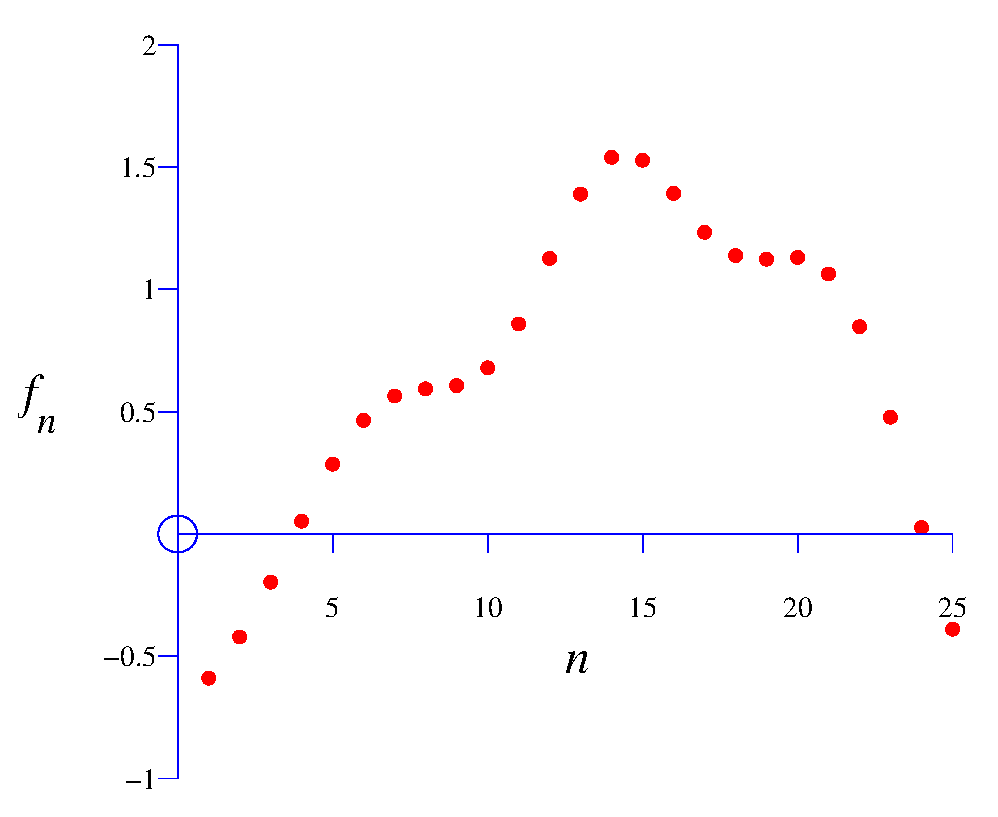
\includegraphics[width=0.45\textwidth]{diagrams/gpSample}}\hfill{}\subfloat[]{

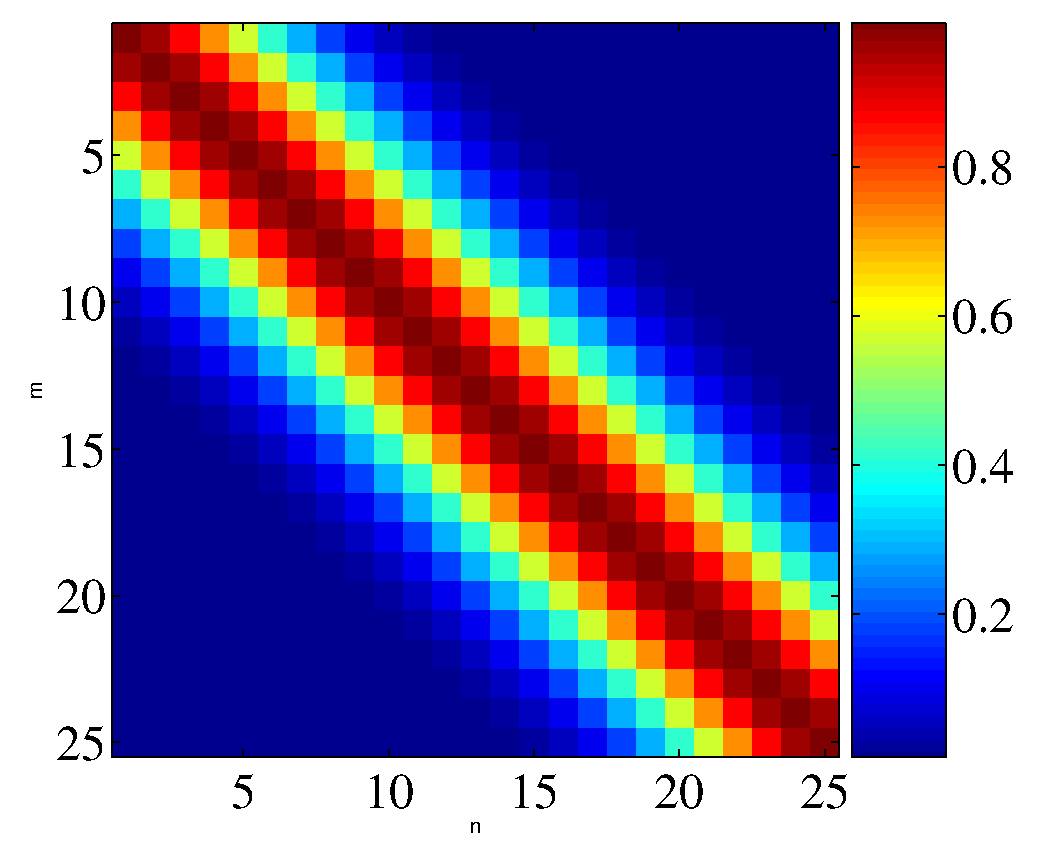
\includegraphics[width=0.45\textwidth]{diagrams/gpCovariance}}

\caption{In (a) we show 25 instantiations of a function, $f_{n}$, as sampled
from a zero mean Gaussian with the covariance matrix given in (b).
In (b) we show the covariance matrix as a greyscale plot. Each element
square in the plot gives the covariance between two points of the
function $f_{n}$ and $f_{m}$. The plots can be recreated with the
command \texttt{demGPSample}.\label{cap:demGPSample}}
\end{figure}

In practice the covariance will not be a function of the indices,
but of an input space $\mathbf{X}$. However, each point in that input
space, $\mathbf{x}_{n}$, will also be indexed by $n$ so for the
moment it is convenient to ignore this relationship.

To see how it is possible to make predictions given the covariance
matrix, let us first consider the covariance of two points. Marginalising
the remaining points leads to a two dimensional Gaussian whose covariance
is made up of the rows and columns from the original covariance associated
with those points. This allows us to plot a contour and visualise
the joint probability over these points. First we take the points
indexed as $f_{1}$ and $f_{2}$. A contour of the joint probability
distribution over this space is shown in Figure~\ref{cap:joint12}(a).
Also, in Figure~\ref{cap:joint12}(c) we visualise the conditional
distribution for $p\left(f_{2}|f_{1},\mathbf{K}\right)$. This can
be viewed as the predictive distribution for $f_{2}$ having observed
$f_{1}$. The strong correlation induced by the covariance, $\mathbf{K}$,
means that the conditional distribution for $f_{2}$ has a mean that
is close to $f_{1}$. 

\begin{figure}
\begin{centering}
\subfloat[]{

\includegraphics[width=0.3\textwidth]{diagrams/demGPCov2D1_2_1}}\hfill{}\subfloat[]{

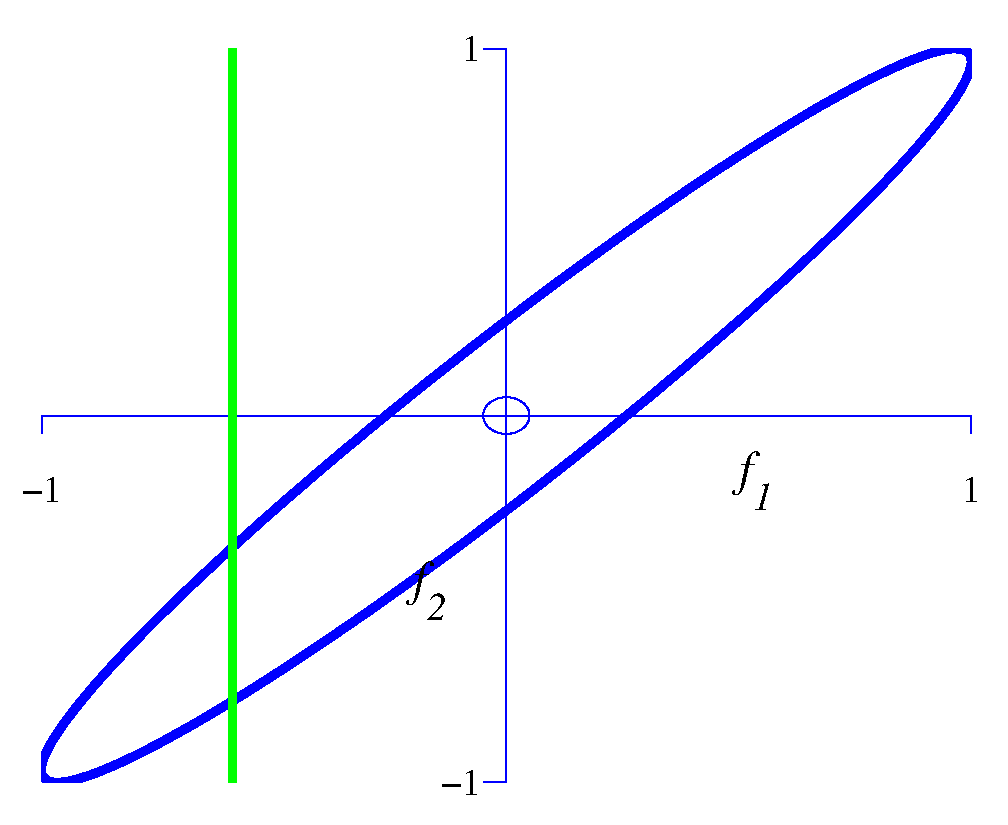
\includegraphics[width=0.3\textwidth]{diagrams/demGPCov2D1_2_2}}\hfill{}\subfloat[]{

\includegraphics[width=0.3\textwidth]{diagrams/demGPCov2D1_2_3}}
\par\end{centering}
\caption{Joint distribution between the values of $f_{1}$ and $f_{2}$: (a)
shows the a single contour (one standard deviation from the mean)
of the Gaussian distribution; (b) shows the instantiated value of
$f_{1}$ as a line dashed in the plot and (c) shows the conditional
distribution of $p\left(f_{2}|f_{1}\right)$ as a dotted line rotated
to be a function of the $f_{2}$-axis of the plot. These plots can
be recreated through the script \texttt{demGPCov2D({[}1 2{]})}. The
portion of the covariance function as computed between these two points
is given by $\mathbf{K}_{12}=\left[\protect\begin{array}{cc}
1 & 0.966\protect\\
0.966 & 1
\protect\end{array}\right]$.\label{cap:joint12}}
\end{figure}

A similar plot is shown in Figure~\ref{cap:joint15} but this time
for the joint distribution between $f_{1}$ and $f_{5}$. The correlation
induced by the covariance function is now much weaker, the conditional
distribution for $f_{5}$ has a mean much closer to zero than that
for $f_{1}$ had.

\begin{figure}
\begin{centering}
\subfloat[]{

\includegraphics[width=0.3\textwidth]{diagrams/demGPCov2D1_5_1}}\hfill{}\subfloat[]{

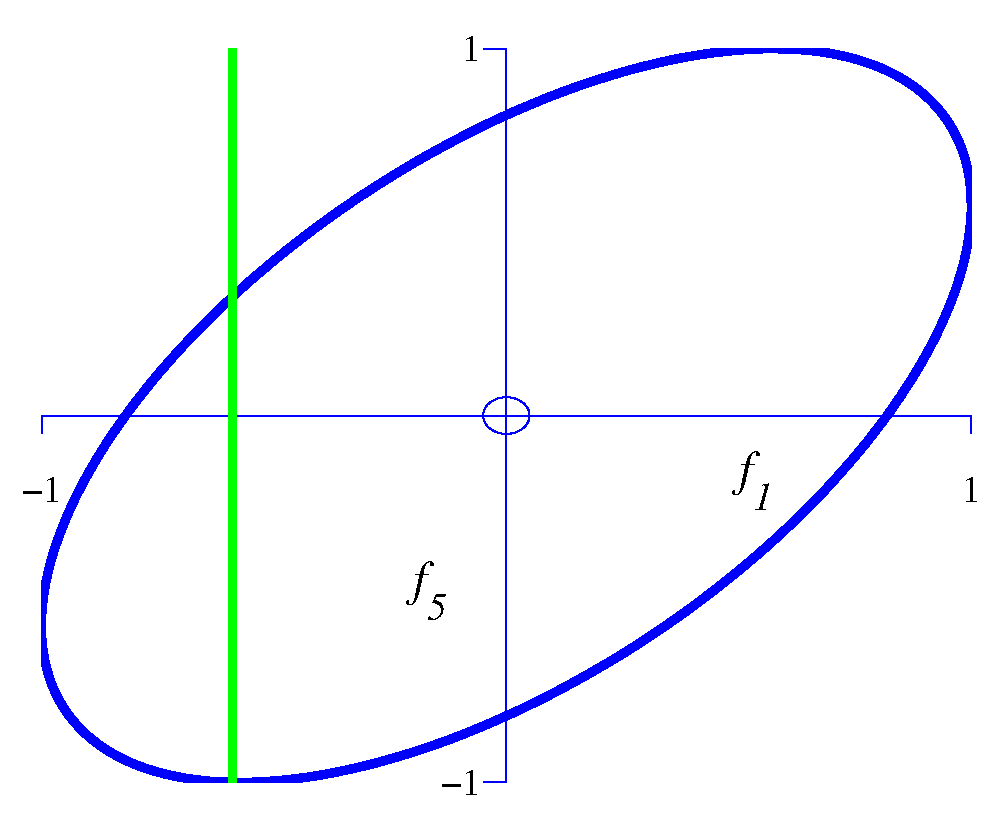
\includegraphics[width=0.3\textwidth]{diagrams/demGPCov2D1_5_2}}\hfill{}\subfloat[]{

\includegraphics[width=0.3\textwidth]{diagrams/demGPCov2D1_5_3}}
\par\end{centering}
\caption{Joint distribution between the values of $f_{1}$ and $f_{5}$: (a)
shows the a single contour (one standard deviation from the mean)
of the Gaussian distribution; (b) shows the instantiated value of
$f_{1}$ as a line dashed in the plot and (c) shows the conditional
distribution of $p\left(f_{5}|f_{1}\right)$ as a dotted line rotated
to be a function of the $f_{5}$-axis of the plot. These plots can
be recreated through the script \texttt{demGPCov2D({[}1 5{]})}. The
portion of the covariance function as computed by these two points
is given by $\mathbf{K}_{15}=\left[\protect\begin{array}{cc}
1 & 0.574\protect\\
0.574 & 1
\protect\end{array}\right]$.\label{cap:joint15}}
\end{figure}

The obvious question is, where does this covariance matrix come from?
In this case the covariance matrix is built using the inputs to the
function $\mathbf{x}_{n}$. The covariance shown in Figure~\label{cap:demGPSample}(b)
is based on Euclidean distance between the points. The input points
used were one dimensional and equally spaced along a line between
-1 and 1. The covariance between points $m$ and $n$ was given by
\begin{equation}
k\left(\mathbf{x}_{m},\mathbf{x}_{n}\right)=\exp\left(-\frac{\gamma}{2}\left(\mathbf{x}_{m}-\mathbf{x}_{n}\right)^{\textrm{T}}\left(\mathbf{x}_{m}-\mathbf{x}_{n}\right)\right),\label{eq:rbfOne}
\end{equation}
where the inverse width parameter $\gamma$ was taken to be 10. Note
that if $m=n$ then the variance of the point is 1. This is why the
furthest extent of the contour at one standard deviation in each of
Figures~\ref{cap:joint12}~and~\ref{cap:joint15} is also one.
This covariance function is known as the radial basis function (RBF),
squared exponential, or Gaussian covariance function. We note that
it shares the same form as the RBF kernel used in support vector machines
\citep{Scholkopf:learning01}. In fact the class of valid covariance
functions is the same as the class of Mercer kernels. We will therefore
use the terms covariance function and kernel interchangeably in what
follows.

The covariance function provides the joint distribution over the instantiations
of the functions. The conditional distribution provides predictions
for as yet unseen locations given points at known locations. This
is analogous to a training set/test set situation in machine learning.
The predictions are locations are on the left hand side of the conditional,
the training data is on the right hand side of the conditional, if
we denote instantiations from the training set as $\mathbf{f}$ and
positions in the test set as $\mathbf{f}_{*}$ we can denote this
conditional as $p\left(\mathbf{f}_{*}|\mathbf{f}\right)$. Since the
joint distribution is Gaussian, we known this conditional distribution
must also be Gaussian. To find the conditional distribution we make
use of a partitioned version of the kernel matrix,
\[
\mathbf{K}=\left[\begin{array}{cc}
\mathbf{K}_{\mathbf{f},\mathbf{f}} & \mathbf{K}_{\mathbf{f},*}\\
\mathbf{K}_{*,\mathbf{f}} & \mathbf{K}_{*,*}
\end{array}\right]
\]
where $\mathbf{K}_{\mathbf{f},\mathbf{f}}$ is the covariance matrix
for the training data points, $\mathbf{f}$, the sub-matrix $\mathbf{K}_{*,*}$
is the covariance matrix for the test data points, $\mathbf{f}_{*}$,
and the sub-matrix $\mathbf{K}_{*,\mathbf{f}}=\mathbf{K}_{\mathbf{f},*}^{\textrm{T}}$
is the cross correlations between training and test data. We are now
in a position to write down the joint distribution of the data via
the partition inverse,
\[
\mathbf{K}^{-1}=\left[\begin{array}{cc}
\mathbf{K}_{\mathbf{f},\mathbf{f}}^{-1}+\mathbf{K}_{\mathbf{f},\mathbf{f}}^{-1}\mathbf{K}_{\mathbf{f},*}\Sigma^{-1}\mathbf{K}_{*,\mathbf{f}}\mathbf{K}_{\mathbf{f},\mathbf{f}}^{-1} & -\mathbf{K}_{\mathbf{f},\mathbf{f}}^{-1}\mathbf{K}_{\mathbf{f},*}\Sigma^{-1}\\
-\Sigma^{-1}\mathbf{K}_{*,\mathbf{f}}\mathbf{K}_{\mathbf{f},\mathbf{f}}^{-1} & \mathbf{\Sigma^{-1}}
\end{array}\right]
\]
where
\[
\Sigma=\mathbf{K}_{*,*}-\mathbf{K}_{*,\mathbf{f}}\mathbf{K_{\mathbf{f},\mathbf{f}}^{-1}}\mathbf{K}_{\mathbf{f},*}.
\]
Through the partitioned inverse we can re-express the joint distribution,
for convenience we write it below as the logarithm of the joint distribution,
\begin{eqnarray*}
\log p\left(\mathbf{f},\mathbf{f}_{*}\right) & = & -\frac{1}{2}\mathbf{f}^{\textrm{T}}\mathbf{K}_{\mathbf{f},\mathbf{f}}^{-1}\mathbf{f}-\frac{1}{2}\mathbf{f}^{\textrm{T}}\mathbf{K}_{\mathbf{f},\mathbf{f}}^{-1}\mathbf{K}_{\mathbf{f},*}\Sigma^{-1}\mathbf{K}_{*,\mathbf{f}}\mathbf{K}_{\mathbf{f},\mathbf{f}}^{-1}\mathbf{f}\\
 &  & +\mathbf{f}\mathbf{K}_{\mathbf{f},\mathbf{f}}^{-1}\mathbf{K}_{\mathbf{f},*}\Sigma^{-1}\mathbf{f}_{*}-\frac{1}{2}\mathbf{f}_{*}^{\textrm{T}}\Sigma^{-1}\mathbf{f}_{*}+\textrm{const}_{1}
\end{eqnarray*}
where the constant term contains portions that are not dependent on
$\mathbf{f}$ or $\mathbf{f}_{*}$. Strictly speaking, the joint distribution
is also conditioned on the parameters of the covariance function,
the training input locations, $\mathbf{X}$, and the test input locations,
$\mathbf{X}_{*}$. This dependence occurs through the kernel functions.
However we are dropping this dependence in what follows to avoid cluttering
the notation. 

The conditional distribution is found by dividing joint distribution
by the prior distribution on $\mathbf{f}$, $p\left(\mathbf{f}\right)=N\left(\mathbf{f}|\mathbf{0},\mathbf{K}_{\mathbf{f},\mathbf{f}}\right)$.
In log space this is equivalent to subtraction of 
\[
\log p\left(\mathbf{f}\right)=\mathbf{-}\frac{1}{2}\mathbf{f}^{\textrm{T}}\mathbf{K}_{\mathbf{f},\mathbf{f}}^{-1}\mathbf{f}+\textrm{const}_{2}
\]
giving 
\begin{eqnarray}
\log p\left(\mathbf{f}_{*}|\mathbf{f}\right) & = & \log p\left(\mathbf{f}_{*},\mathbf{f}\right)-\log p\left(\mathbf{f}\right)\nonumber \\
 & = & -\frac{1}{2}\mathbf{f}^{\textrm{T}}\mathbf{K}_{\mathbf{f},\mathbf{f}}^{-1}\mathbf{K}_{\mathbf{f},*}\Sigma^{-1}\mathbf{K}_{*,\mathbf{f}}\mathbf{K}_{\mathbf{f},\mathbf{f}}^{-1}\mathbf{f}+\mathbf{f}^{\textrm{T}}\mathbf{K}_{\mathbf{f},\mathbf{f}}^{-1}\mathbf{K}_{\mathbf{f},*}\Sigma\mathbf{f}_{*}\nonumber \\
 &  & -\frac{1}{2}\mathbf{f}_{*}^{\textrm{T}}\Sigma^{-1}\mathbf{f}_{*}+\textrm{const}_{1}-\textrm{const}_{2}\label{eq:thirdLineConditional}\\
 & = & -\frac{1}{2}\left(\mathbf{f}_{*}-\mathbf{K}_{*,\mathbf{f}}\mathbf{K}_{\mathbf{f},\mathbf{f}}^{-1}\mathbf{f}\right)^{\textrm{T}}\mathbf{\Sigma^{-1}}\left(\mathbf{f}_{*}-\mathbf{K}_{*,\mathbf{f}}\mathbf{K}_{\mathbf{f},\mathbf{f}}^{-1}\mathbf{f}\right)\nonumber \\
 &  & +\textrm{const}_{3}\label{eq:fifthLineConditional}\\
 & = & \log N\left(\mathbf{f}_{*}|\mathbf{\bar{\mathbf{f}}}_{*},\Sigma\right).\label{eq:gpConditional}
\end{eqnarray}
where $\bar{\mathbf{f}}=\mathbf{K}_{*,\mathbf{f}}\mathbf{K}_{\mathbf{f},\mathbf{f}}^{-1}\mathbf{f}$,
$\textrm{const}_{3}=\textrm{const}_{1}-\textrm{const}_{2}$ and (\ref{eq:fifthLineConditional})
is derived from (\ref{eq:thirdLineConditional}) by completing the
square. 

So we can see that if we observe points from the function, \textbf{$\mathbf{f}$},
directly for a given set of training data $\mathbf{X}$ then we can
predict the locations of functions at as yet unseen locations whose
inputs are given by $\mathbf{X}_{*}$. The resulting distribution
is also a Gaussian process, but with a mean given by $\bar{\mathbf{f}}$
and a covariance given by $\Sigma$. In general though, we will not
make direct observations of the function, our observations are more
likely to be corrupted by noise. We therefore also define a noise
model $p\left(\mathbf{y}|\mathbf{f}\right)$ which relates our actual
observations, $\mathbf{y}$, to the function $\mathbf{f}$ (see Figure~\ref{cap:gpGraph}).
A standard noise model for regression is independent Gaussian random
noise. In this case we can write the noise model as
\begin{equation}
p\left(\mathbf{y}|\mathbf{f}\right)=\prod_{n=1}^{N}p\left(y_{n}|f_{n}\right)=\prod_{n=1}^{N}N\left(y_{n}|f_{n},\beta^{-1}\right),\label{eq:gpGaussNoise}
\end{equation}
\emph{i.e}. we are assuming that the function becomes corrupted by
the addition of independent Gaussian noise with a precision of $\beta^{-1}$
at each observation. Given the Gaussian noise model in (\ref{eq:gpGaussNoise})
computation of the marginal likelihood, 
\[
p\left(\mathbf{y}\right)=\int p\left(\mathbf{y}|\mathbf{f}\right)p\left(\mathbf{f}\right)d\mathbf{f},
\]
is straightforward,
\begin{eqnarray}
p\left(\mathbf{y}\right) & \propto & \int\exp\left(-\frac{\beta}{2}\left(\mathbf{y}-\mathbf{f}\right)^{\textrm{T}}\left(\mathbf{y}-\mathbf{f}\right)-\frac{1}{2}\mathbf{f}^{\textrm{T}}\mathbf{K}_{\mathbf{f},\mathbf{f}}^{-1}\mathbf{f}\right)d\mathbf{f}\nonumber \\
 & \propto & \int\exp\left(-\frac{\beta}{2}\mathbf{y}^{\textrm{T}}\mathbf{y}-\frac{1}{2}\mathbf{f}^{\textrm{T}}\left(\mathbf{K}_{\mathbf{f},\mathbf{f}}^{-1}+\beta\mathbf{I}\right)\mathbf{f}+\beta\mathbf{y}^{\textrm{T}}\mathbf{f}\right)d\mathbf{f}\label{eq:marginalSecondLine}\\
 & \propto & \exp\left(-\frac{1}{2}\mathbf{y}^{\textrm{T}}\left(\mathbf{\beta I}-\beta^{2}\left(\mathbf{K}_{\mathbf{f},\mathbf{f}}^{-1}+\beta\mathbf{I}\right)^{-1}\right)\mathbf{y}\right)\label{eq:marginalThirdLine}\\
 & \propto & \exp\left(-\frac{1}{2}\mathbf{y}^{\textrm{T}}\left(\mathbf{K}_{\mathbf{f},\mathbf{f}}+\beta^{-1}\mathbf{I}\right)^{-1}\mathbf{y}\right)\label{eq:marginalFourthLine}\\
 & = & N\left(\mathbf{y}|\mathbf{0},\mathbf{K}_{\mathbf{f},\mathbf{f}}+\beta^{-1}\mathbf{I}\right),\label{eq:gaussianMarginal}
\end{eqnarray}
where the integral in (\ref{eq:marginalSecondLine}) can again be
undertaken through standard Gaussian results \citep[Appendix B]{Bishop:book95}
and we move from (\ref{eq:marginalThirdLine}) to (\ref{eq:marginalFourthLine})
through inspection by recognising the form of the matrix inversion
lemma in (\ref{eq:marginalThirdLine}). The resulting marginal likelihood
is then a Gaussian process on $\mathbf{y}$ with a modified covariance
function of the form $\mathbf{\hat{K}}_{\mathbf{y},\mathbf{y}}=\mathbf{K}_{\mathbf{f},\mathbf{f}}+\beta^{-1}\mathbf{I}$. 

\subsection{Summing Covariance Functions}

As an aside we note that the form of $p\mathbf{\left(\mathbf{y}|\mathbf{f}\right)}$
can also be seen as a Gaussian process over $\mathbf{y}$ with a given
mean $\mathbf{f}$ and a covariance function $\mathbf{K}_{\mathbf{y},\mathbf{y}}=\beta^{-1}\mathbf{I}$.
The particular form of this covariance function is that all points
are uncorrelated, \emph{i.e.} the process is just white noise. However
regardless of the form of the covariance function the result of the
marginalisation above would remain the same, 
\[
N\left(\mathbf{y}|\mathbf{0},\mathbf{K}_{\mathbf{f},\mathbf{f}}+\mathbf{K}_{\mathbf{y},\mathbf{y}}\right)=\int N\left(\mathbf{y}|\mathbf{f},\mathbf{K}_{\mathbf{y},\mathbf{y}}\right)N\left(\mathbf{f}|\mathbf{0},\mathbf{K}_{\mathbf{f},\mathbf{f}}\right)d\mathbf{f},
\]
so we see that a new covariance function can be generated by adding
two different covariance functions together. This has the interpretation
of a hierarchical Gaussian process, where the mean of each process
is itself treated as a Gaussian process. 

\subsection{Parameters of the Covariance Function}

The covariance function we described in (\ref{eq:rbfOne}) has a parameter:
the inverse width. We also saw from the contour plots of the correlation
between the points, that the maximum standard deviation was unity.
If we wish to have a covariance function that existed on a non unit
scale we need to introduce a further parameter, $\alpha$,
\begin{equation}
k\left(\mathbf{x}_{m},\mathbf{x}_{n}\right)=\alpha\exp\left(-\frac{\gamma}{2}\left(\mathbf{x}_{m}-\mathbf{x}_{n}\right)^{\textrm{T}}\left(\mathbf{x}_{m}-\mathbf{x}_{n}\right)\right),\label{eq:rbfTwo}
\end{equation}
which controls the variance of the function. Note that this parameter
$\alpha$ is analogous to $\beta^{-1}$ (which controls the variance
of the white noise process). Here $\alpha$ is controlling the variance
of the function generated by the RBF kernel. In the context of the
marginal distribution over $\mathbf{y}$,
\begin{equation}
p\left(\mathbf{y}|\alpha,\beta,\gamma\right)=N\left(\mathbf{y}|\mathbf{0},\mathbf{K}_{\mathbf{f},\mathbf{f}}+\mathbf{\beta}^{-1}\mathbf{I}\right),\label{eq:gpMarginal2}
\end{equation}
 where we have made explicit the dependence of the marginal likelihood
on $\alpha$, $\beta$ and $\gamma$. This dependence occurs through
$\mathbf{K}_{\mathbf{f},\mathbf{f}}$, the elements of which are given
by (\ref{eq:rbfTwo}), we can view $\sqrt{\alpha\beta}$ as a signal
to noise ratio. The standard deviation of the signal is $\sqrt{\alpha}$
and the standard deviation of the noise is $\sqrt{\beta^{-1}}$. In
many kernel methods, these parameters must be selected through cross
validation. An advantage of the Gaussian process point of view is
that they can be optimised by maximisation of the marginal likelihood
$p\left(\mathbf{y}|\alpha,\beta,\gamma\right)$. This is known as
empirical Bayes or type II maximum likelihood. Priors can also be
placed over these parameters and sampling used to estimate their posteriors
(see \emph{e.g.}\citealt{Williams:Gaussian96}). 

\subsection{Different Covariance Functions\label{subsec:covarianceFunctions}}

By changing the characteristics of the covariance function we can
sample different functions from the prior. For example, setting each
element of the kernel matrix to an inner product between the points,
\[
k\left(\mathbf{x}_{m},\mathbf{x}_{n}\right)=\alpha\mathbf{x}_{m}^{\textrm{T}}\mathbf{x}_{n},
\]
produces functions that are linear. Note that this kernel function
can also be written as
\[
\mathbf{K}_{\mathbf{f},\mathbf{f}}=\mathbf{X}\mathbf{X}^{\textrm{T}}.
\]
 \citet{Williams:infinite96} showed that a multi-layer perceptron
with infinite hidden nodes has a covariance function of the form
\[
k\left(\mathbf{x}_{m},\mathbf{x}_{n}\right)=\alpha\textrm{sin}^{-1}\left(\frac{w\mathbf{x}_{m}^{\textrm{T}}\mathbf{x}_{n}+b}{\sqrt{w\mathbf{x}_{m}^{\textrm{T}}\mathbf{x}_{m}+b+1}\sqrt{w\mathbf{x}_{n}^{\textrm{T}}\mathbf{x}_{n}+b+1}}\right),
\]
where a Gaussian prior over the weights from the input to hidden units
is used with a variance $w$ and a prior over the locations of the
activation functions with variance $b$. 

Finally a constant offset in the function can be accounted for by
adding a kernel function which is constant in value. 
\[
k\left(\mathbf{x}_{m},\mathbf{x}_{n}\right)=\alpha,
\]
we will refer to this as the bias kernel. We show some examples of
samples associated with tese covariance functions in Figure~\ref{cap:kernelSamples}

\begin{figure}
\subfloat[]{

\includegraphics[width=0.3\textwidth]{diagrams/demCovFuncSample1}}\hfill{}\subfloat[]{

\includegraphics[width=0.3\textwidth]{diagrams/demCovFuncSample2}}\hfill{}\subfloat[]{

\includegraphics[width=0.3\textwidth]{diagrams/demCovFuncSample3}}

\subfloat[]{

\includegraphics[width=0.3\textwidth]{diagrams/demCovFuncSample4}}\hfill{}\subfloat[]{

\includegraphics[width=0.3\textwidth]{diagrams/demCovFuncSample5}}\hfill{}\subfloat[]{

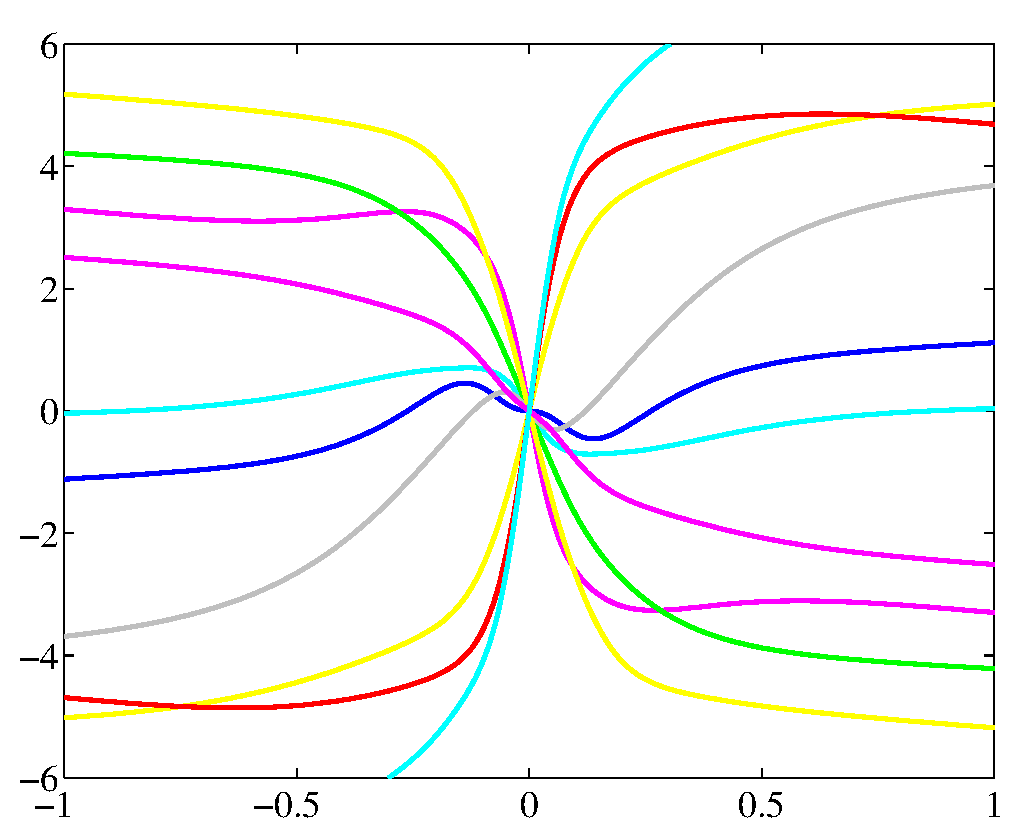
\includegraphics[width=0.3\textwidth]{diagrams/demCovFuncSample6}}

\subfloat[]{

\includegraphics[width=0.3\textwidth]{diagrams/demCovFuncSample7}}\hfill{}\subfloat[]{

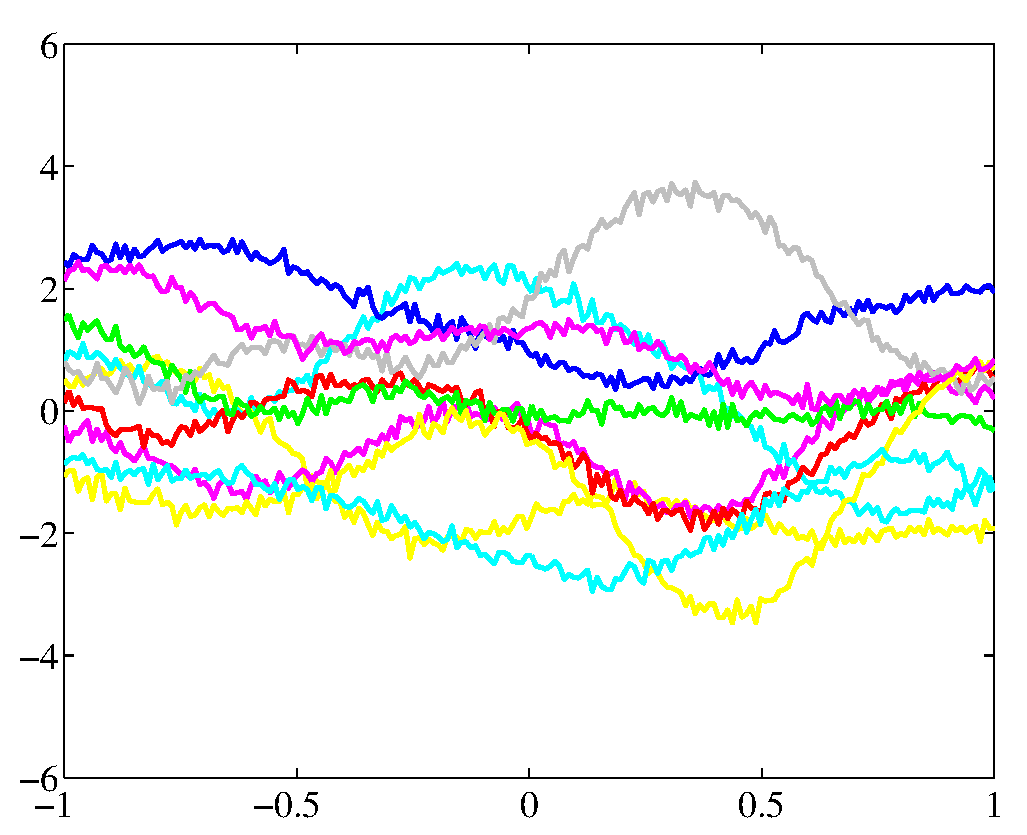
\includegraphics[width=0.3\textwidth]{diagrams/demCovFuncSample8}}

\caption{Samples from different covariance functions. (a) RBF kernel with $\gamma=10$,
$\alpha=1$, (b) RBF kernel with $\gamma=1$, $\alpha=1$ (c) RBF
kernel with $\gamma=10$, $\alpha=4$, (d) linear kernel with $\alpha=16$,
(e) MLP kernel with $\alpha=8$, $w=100$ and $b=100$, (f) MLP kernel
with $\alpha=8$, $b=0$ and $w=100$, (g) bias kernel with $\alpha=1$
and (h) Summed combination of: RBF kernel, $\alpha=1$, $\gamma=10$;
bias kernel, $\alpha=$1; and white noise kernel, $\beta=100$. Samples
can be recreated with the script \texttt{demCovFuncSample}.\label{cap:kernelSamples}}
\end{figure}


\subsection{Consistency}

Gaussian processes are consistent in that the posterior predictions
at each point remain the same regardless of the number and location
of the test points. To see this we first consider an additional set
of test points $\mathbf{f}_{+}$ which is disjoint from $\mathbf{f}_{*}$.
The conditional probability of our original test points can be expressed
as 
\[
p\left(\mathbf{f}_{*}|\mathbf{f}\right)=\int p\left(\mathbf{f}_{*},\mathbf{f}_{+}|\mathbf{f}\right)d\mathbf{f}_{+},
\]
for the system to be consistent this marginal likelihood must be the
same regardless of $\mathbf{f}_{+}$. In other words, if we replaced
$\mathbf{f}_{+}$ with $\hat{\mathbf{f}}_{+}$ we would require
\[
p\left(\mathbf{f}_{*}|\mathbf{f}\right)=\int p\left(\mathbf{f}_{*},\mathbf{f}_{+}|\mathbf{f}\right)d\mathbf{f}_{+}=\int p\left(\mathbf{f}_{*},\hat{\mathbf{f}}_{+}|\mathbf{f}\right)d\hat{\mathbf{f}}_{+}
\]
where $\hat{\mathbf{f}}_{+}\neq\mathbf{f}_{+}$.

\subsection{Summary}

We have reviewed some of the salient points of Gaussian processes,
in particular we have shown how a Gaussian process arises from the
specification of a covariance function. Given a sub-set of observations
of a function, and an associated covariance, we can make predictions
about the the likely location of the function in regions where we
hadn't previously observed data. 

The parameters of the covariance function can be found through maximisation
of the marginal likelihood (\ref{eq:gpMarginal2}).

\section{The GP-LVM\label{sec:GPLVM}}

The standard probabilistic interpretation of PCA we reviewed in Section~\ref{sec:PPCA}
combines a Gaussian likelihood, 
\[
p\left(\mathbf{Y}|\mathbf{W},\mathbf{X},\beta\right)=\prod_{n=1}^{N}N\left(\mathbf{y}_{n}|\mathbf{Wx}_{n},\beta^{-1}\mathbf{I}\right)
\]
with a Gaussian prior on the latent variables, $\mathbf{X}$. The
GP-LVM takes a different perspective on the model. Rather than marginalising
the latent variables, we seek to marginalise the mapping. Graphically,
we can depict the two different approaches as shown in Figure~\ref{cap:probabilisticPCAGraph}.

\begin{figure}
\includegraphics[width=0.35\textwidth]{diagrams/ppcaGraph}\hfill{}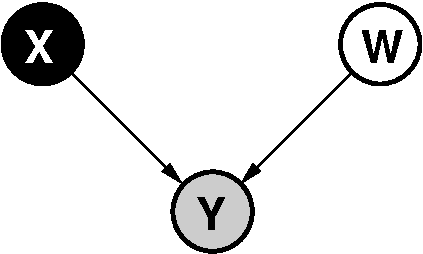
\includegraphics[width=0.35\textwidth]{diagrams/gplvmGraph}

\caption{Graphical representation of (a) the standard probabilistic PCA model
and (b) its dual representation which also leads to a probabilistic
interpretation of PCA. The nodes are shaded to represent different
treatments. \emph{Black} shaded nodes are optimised, \emph{white}
shaded nodes are marginalised and \emph{grey} shaded nodes are observed
variables.\label{cap:probabilisticPCAGraph}}
\end{figure}

As we shall see this approach will lead to a dual representation of
probabilistic PCA. The required marginalisation now takes the form
\[
p\left(\mathbf{Y}|\mathbf{X},\beta\right)=\int\prod_{n=1}^{N}p\left(\mathbf{y}_{n}|\mathbf{x}_{n},\mathbf{W},\beta\right)p\left(\mathbf{W}\right)d\mathbf{W}.
\]
By specifying a Gaussian prior distribution over the parameters of
the mapping, 
\[
p\left(\mathbf{W}\right)=\prod_{i}N\left(\mathbf{w}_{i}|\mathbf{0},\mathbf{I}\right)
\]
 where $\mathbf{w}_{i}$ is the $i$th row of the matrix $\mathbf{W}$,
and then integrating over $\mathbf{W}$ we obtain a marginalised likelihood
for $\mathbf{Y}$, 
\begin{equation}
p\left(\mathbf{Y}|\mathbf{X},\beta\right)=\frac{1}{\left(2\pi\right)^{\frac{DN}{2}}\left|\mathbf{K}\right|^{\frac{D}{2}}}\exp\left(-\frac{1}{2}\textrm{tr}\left(\mathbf{K}^{-1}\mathbf{YY}^{\textrm{T}}\right)\right),\label{eq:appDualPPCAMarginal}
\end{equation}
where $\mathbf{K}=\mathbf{XX}^{\textrm{T}}+\beta^{-1}\mathbf{I}$
and $\mathbf{X}=\left[\mathbf{x}_{1}^{\textrm{T}}\dots\mathbf{x}_{N}^{\textrm{T}}\right]^{\textrm{T}}$.
The structure of this model is shown in \ref{cap:probabilisticPCAGraph}(b).
Note that with our earlier definition of $\mathbf{C}=\mathbf{W}\mathbf{W}^{\textrm{T}}+\beta^{-1}\mathbf{I}$
we can write the marginal likelihood for standard PPCA (\ref{eq:ppcaMarginaLikelihood})
as
\[
p\left(\mathbf{Y}|\mathbf{W},\beta\right)=\frac{1}{\left(2\pi\right)^{\frac{DN}{2}}\left|\mathbf{C}\right|^{\frac{N}{2}}}\exp\left(-\frac{1}{2}\textrm{tr}\left(\mathbf{C}^{-1}\mathbf{Y}^{\textrm{T}}\mathbf{Y}\right)\right),
\]
 which highlights to a greater extent the duality between (\ref{eq:appDualPPCAMarginal})
and (\ref{eq:ppcaMarginaLikelihood}). Optimisation of (\ref{eq:appDualPPCAMarginal})
is clearly highly related to optimisation of (\ref{eq:ppcaMarginaLikelihood}).
\citet{Tipping:probpca99} showed how to optimise (\ref{eq:ppcaMarginaLikelihood}),
in the next section we review this optimisation for DPPCA, but generalise
it slightly so that it applies for any positive definite matrix \textbf{$\mathbf{S}$},
rather than only the inner product matrix $\mathbf{Y}\mathbf{Y}^{\textrm{T}}$.
First though we make the connection to Gaussian processes by highlighting
the fact that (\ref{eq:appDualPPCAMarginal}) can be written as
\begin{equation}
p\left(\mathbf{Y}|\mathbf{X},\beta\right)=\prod_{i=1}^{D}\frac{1}{\left(2\pi\right)^{\frac{N}{2}}\left|\mathbf{K}\right|^{\frac{1}{2}}}\exp\left(-\frac{1}{2}\mathbf{y}_{:,i}^{\textrm{T}}\mathbf{K}^{-1}\mathbf{y}_{:,i}\right),\label{eq:gplvmLikelihood}
\end{equation}
here $\mathbf{y}_{:,i}$ is the $i$th column of $\mathbf{Y}$. This
likelihood is thus recognised as a product of $D$ independent Gaussian
processes, each process being associated with a different dimension
of the data set. However, here we are suggesting maximising over $\mathbf{X}$
as well as the kernel parameters. If $q>D$ this maximisation would
not be well determined, but as long as $q<D$ we are obtaining a reduced
dimensional representation of our data. We will now show how, for
the case of a linear covariance matrix, this model is equivalent to
PCA.

\subsection{Maximisation of the Marginal Likelihood}

The proof of the maximum likelihood solution for dual probabilistic
PCA closely mirrors that given in \citet{Tipping:probpca99}, we include
it here for completeness. For a more general proof see \citet{Lawrence:matching04}.
Maximising (\ref{eq:appDualPPCAMarginal}) is equivalent to minimising
its negative logarithm, 
\begin{equation}
L=\frac{N}{2}\ln2\pi+\frac{1}{2}\ln\left|\mathbf{K}\right|+\frac{1}{2}\textrm{tr}\left(\mathbf{K}^{-1}\mathbf{S}\right),\label{eq:negEigObjective}
\end{equation}
where $\mathbf{S}=D^{-1}\mathbf{Y}\mathbf{Y}^{\textrm{T}}$. The gradient
of the negative log likelihood with respect to $\mathbf{X}$ can be
found as
\[
\frac{\partial L}{\partial\mathbf{X}}=-\mathbf{K}^{-1}\mathbf{S}\mathbf{K}^{-1}\mathbf{X}+\mathbf{K}^{-1}\mathbf{X},
\]
setting the equation to zero and pre-multiplying by $\mathbf{K}$
gives
\[
\mathbf{S}\left[\beta^{-1}\mathbf{I}+\mathbf{XX}^{\textrm{T}}\right]^{-1}\mathbf{X}=\mathbf{X}.
\]
We substitute $\mathbf{X}$ with its singular value decomposition,
$\mathbf{X}=\mathbf{ULV}^{\textrm{T}}$, giving
\[
\mathbf{SU}\left[\mathbf{L}+\beta^{-1}\mathbf{L}^{-1}\right]^{-1}\mathbf{V}^{\textrm{T}}=\mathbf{U}\mathbf{LV}^{\textrm{T}}
\]
Right multiplying both sides by $\mathbf{V}$ (note that the solution
is invariant to $\mathbf{V}$) we have, after some rearrangement,
\[
\mathbf{SU}=\mathbf{U}\left(\beta^{-1}\mathbf{I}+\mathbf{L}^{2}\right),
\]
which, since $\left(\beta^{-1}\mathbf{I}+\mathbf{L}^{2}\right)$ is
diagonal can be solved by an eigenvalue problem where $\mathbf{U}$
are eigenvectors of $\mathbf{S}$ and $\Lambda=\left(\beta^{-1}\mathbf{I}+\mathbf{L}^{2}\right)$
are the eigenvalues. This implies that the elements from the diagonal
of $\mathbf{L}$ are given by 
\begin{equation}
l_{i}=\left(\lambda_{i}-\beta^{-1}\right)^{\frac{1}{2}}.\label{eq:XeigenvalueUpdate}
\end{equation}
 

\subsection{The Retained Eigenvalues}

If $q<D$ we must select which eigenvectors to retain, all eigenvectors
are associated with stationary points, so how do we choose which to
retain? For convenience let us ignore our previously defined ordering
of the eigenvalues in terms of their magnitude and assume that we
keep the first $q$ eigenvalues. 

First note that
\[
\mathbf{K}=\mathbf{U}\left[\mathbf{L}^{2}+\beta^{-1}\mathbf{I}\right]\mathbf{U}^{\textrm{T}}
\]
where $\mathbf{U}$ is all the eigenvectors of \textbf{$\mathbf{S}$}.
The Kullback Leibler (KL) divergence between zero mean Gaussians with
covariances given by $\mathbf{K}$ and $\mathbf{S}$ given by (\ref{eq:negEigObjective})
minus the log determinant of $\mathbf{S}$, which is constant in $\mathbf{X}$.
Minimising this KL divergence is thus equivalent to minimising (\ref{eq:negEigObjective}).
\begin{eqnarray*}
\textrm{KL}\left(\mathbf{S}||\mathbf{K}\right) & = & \frac{1}{2}\ln\left|\mathbf{K}\right|-\frac{1}{2}\ln\left|\mathbf{S}\right|+\frac{1}{2}\textrm{tr}\left(\mathbf{K}^{-1}\mathbf{S}\right)-\frac{N}{2}\\
 & = & \frac{1}{2}\sum_{i=1}^{q}\ln\lambda_{i}-\frac{N-q}{2}\ln\beta-\frac{1}{2}\sum_{i=1}^{N}\ln\lambda_{i}+\frac{1}{2}\textrm{tr}\left(\left[\mathbf{L}^{2}+\beta^{-1}\mathbf{I}\right]^{-1}\Lambda\right)\\
 & = & -\frac{1}{2}\sum_{i=q+1}^{N}\ln\lambda_{i}-\frac{N-q}{2}\ln\beta-\frac{N-q}{2}+\frac{\beta}{2}\sum_{i=q+1}^{N}\lambda_{i}
\end{eqnarray*}
where we have used the fact that $\mathbf{S}=\mathbf{U}\Lambda\mathbf{U}^{\textrm{T}}$.
Differentiating with respect to $\beta$ and setting the result to
zero to obtain a fixed point equation then gives
\[
\beta=\frac{N-q}{\sum_{i=q+1}^{N}\lambda_{i}}
\]
which when substituted back leads to 
\begin{equation}
\textrm{KL}\left(\mathbf{S}||\mathbf{K}\right)=\frac{N-q}{2}\left(\ln\frac{\sum_{i=q+1}^{N}\lambda_{i}}{N-q}-\frac{1}{N-q}\sum_{i=q+1}^{N}\ln\lambda_{i}\right),\label{eq:pdObjective}
\end{equation}
which is recognised as the difference between the log ratio of the
arithmetic and geometric means of the discarded eigenvalues. This
difference will be zero if and only if the discarded eigenvalues are
constant (when the arithmetic and geometric means become equal) otherwise
it is positive. The difference is minimised by ensuring that the eigenvalues
we discard are adjacent to each other in terms of magnitude. 

Which eigenvalues should we then discard? From (\ref{eq:XeigenvalueUpdate})
we note that the retained eigenvalues must be larger than $\beta$,
otherwise $l_{i}$ will be complex. The only way this can be true
is if we discard the smallest $N-q$ eigenvalues.

\subsection{Equivalence of Eigenvalue Problems\label{sec:equivEigenvalue}}

In Section~\ref{sec:PPCA} we reviewed probabilistic PCA, here we
have introduced a new dual version of probabilistic PCA which leads
to a different eigenvalue problem. However, these eigenvalue problems
are equivalent as we shall now show. For DPPCA the eigenvalue problem
is of the form
\[
\mathbf{YY}^{\textrm{T}}\mathbf{U}=\mathbf{U}\Lambda.
\]
Premultiplying by $\mathbf{Y}^{\textrm{T}}$ then gives 
\begin{equation}
\mathbf{Y}^{\textrm{T}}\mathbf{YY}^{\textrm{T}}\mathbf{U}=\mathbf{Y}^{\textrm{T}}\mathbf{U}\Lambda\label{eq:covarianceEigenProblem}
\end{equation}
Since $\mathbf{U}$ is the eigenvectors of $\mathbf{Y}\mathbf{Y}^{\textrm{T}}$
(see the previous section) the matrix $\mathbf{U}^{\textrm{T}}\mathbf{YY}^{\textrm{T}}\mathbf{U}=\Lambda$,
therefore matrix $\mathbf{U}^{\prime}=\mathbf{Y}^{\textrm{T}}\mathbf{U}\Lambda^{-\frac{1}{2}}$
is orthonormal. Post multiplying both sides of (\ref{eq:covarianceEigenProblem})
by $\Lambda^{-\frac{1}{2}}$ gives
\[
\mathbf{Y}^{\textrm{T}}\mathbf{YU}^{\prime}=\mathbf{U}^{\prime}\Lambda
\]
which is recognised as the form of the eigenvalue problem associated
with PPCA as given in (\ref{eq:ppcaEigenValueProblem}), where the
eigenvectors of $\mathbf{Y}^{\textrm{T}}\mathbf{Y}$ are given by
$\mathbf{U}^{\prime}=\mathbf{Y}^{\textrm{T}}\mathbf{U}\Lambda^{-\frac{1}{2}}$
and the eigenvalues are given by $\Lambda$ (as they were for DPPCA).

\section{Non-linear GP-LVM\label{sec:GP-LVMalgorithmic}}

We saw in the previous section how PCA can be interpreted as a product
of Gaussian processes that maps latent-space points to points in data-space.
The positions of the points in the latent-space can be determined
by maximising the process likelihood with respect to $\mathbf{X}$.
It is natural, therefore, to consider alternative GP-LVMs by introducing
covariance functions which allow for non-linear processes. The resulting
models will not, in general, be optimisable through an eigenvalue
problem. 
\begin{figure}
\begin{centering}
\includegraphics[width=0.35\textwidth]{diagrams/gpGraphGPLVM}
\par\end{centering}
\caption{The Gaussian process as a latent variable model, now both kernel parameters,
$\boldsymbol{\theta}$ and latent positions are optimised. \label{cap:gplvmGraph}}
\end{figure}


\subsection{Optimisation of the Non-linear Model}

In Section~\ref{sec:GPLVM} we saw for the linear kernel that a closed
form solution for dual PPCA could be obtained up to an arbitrary rotation
matrix. For non-linear kernels, such as the RBF kernel and MLP kernel
discussed in Section~\ref{subsec:covarianceFunctions} there will
be no such closed form solution and there are likely to be multiple
local optima. To use a particular kernel in the GP-LVM we first note
that gradients of (\ref{eq:gpMarginal2}) with respect to the latent
points can be found through first taking the gradient with respect
to the kernel, 
\begin{equation}
\frac{\partial L}{\partial\mathbf{K}}=\mathbf{K}^{-1}\mathbf{YY}^{\textrm{T}}\mathbf{K}^{-1}-D\mathbf{K}^{-1},\label{eq:likelihoodGradK}
\end{equation}
and then combining it with $\frac{\partial\mathbf{K}}{\partial x_{n,j}}$
through the chain rule. As computation of (\ref{eq:likelihoodGradK})
is straightforward and independent of the kernel choice we only require
that the gradient of the kernel with respect to the latent points
can be computed. These gradients may then be used in combination with
(\ref{eq:gpMarginal2}) in a non-linear optimiser to obtain a latent
variable representation of the data. Furthermore, gradients with respect
to the parameters of the kernel matrix may be computed and used to
jointly optimise $\mathbf{X}$ and the kernel's parameters. 

The log-likelihood is a highly non-linear function of the embeddings
and the parameters. We are therefore forced to turn to gradient based
optimisation of the objective function. In all our experiments we
made use of conjugate gradients or the scaled conjugate gradient \citep{Moller:scg93}
algorithm.

\subsection{Illustration of GP-LVM via SCG\label{subsec:IllustrationGP-LVM}}

To illustrate the Gaussian process latent variable model we now make
use of the `multi-phase oil flow' data \citep{Bishop:oil93}. This
is a twelve dimensional data set containing data of three known classes
corresponding to the phase of flow in an oil pipeline: stratified,
annular and homogeneous. In \citet{Bishop:gtmncomp98} this data was
used to demonstrate the GTM algorithm. Here we use a sub-sampled version
of the data (containing 100 data points) to demonstrate the fitting
of a GP-LVM with a simple radial basis function (RBF) kernel.

As we saw in Section~\ref{sec:GPLVM}, seeking a lower dimensional
embedding with PCA is equivalent to a GP-LVM model with a linear kernel,
\[
k\left(\mathbf{x}_{n},\mathbf{x}_{m}\right)=\mathbf{x}_{n}^{\textrm{T}}\mathbf{x}_{m}+\beta^{-1}\delta_{nm},
\]
where $\delta_{ij}$ is the Kronecker delta function. 

For comparison we visualised the data set using several of the approaches
mentioned in the introduction. In Figure~\ref{cap:oilVisualisation100}(a)
we show the first two principal components of the data. Figure~\ref{cap:oilVisualisation100}(b)
then shows the visualisation obtained using the GP-LVM with the RBF
kernel,
\[
k\left(\mathbf{x}_{i},\mathbf{x}_{j}\right)=\alpha_{\textrm{rbf}}\exp\left(-\frac{\gamma}{2}\left(\mathbf{x}_{i}-\mathbf{x}_{j}\right)^{\textrm{T}}\left(\mathbf{x}_{i}-\mathbf{x}_{j}\right)\right)+\alpha_{\textrm{bias}}+\beta^{-1}\delta_{ij}.
\]
To obtain this visualisation the log likelihood was optimised jointly
with respect to the latent positions $\mathbf{X}$ and the kernel
parameters $\alpha_{\textrm{bias}},\,\alpha_{\textrm{rbf}}$, $\beta$
and $\gamma$. The kernel was initialised using PCA to set $\mathbf{X}$,
the kernel parameters were initialised as $\alpha_{\textrm{rbf}}=\gamma=1$
and $\beta^{-1}=\alpha_{\textrm{bias}}=\exp\left(-1\right)$.

Note that there is a redundancy in the representation between the
overall scale of the matrix $\mathbf{X}$ and the value of $\gamma$.
This redundancy was removed by penalising the log likelihood with
half the sum of the squares of each element of $\mathbf{X}$: this
implies we were actually seeking a MAP solution\footnote{Multiplying the likelihood by this prior leads to a joint distribution
over data points and latent points. As a function of $\mathbf{X}$
this joint distribution is proportional to the posterior distribution
$p\left(\mathbf{X}|\mathbf{Y}\right)$, therefore maximising the joint
distribution is equivalent to seeking a MAP solution.} with a Gaussian prior for $\mathbf{X}$,
\[
p\left(\mathbf{X}\right)=\prod_{n=1}^{N}N\left(\mathbf{x}_{n}|\mathbf{0},\mathbf{I}\right).
\]
 

\begin{figure}
\begin{centering}
\subfloat[]{

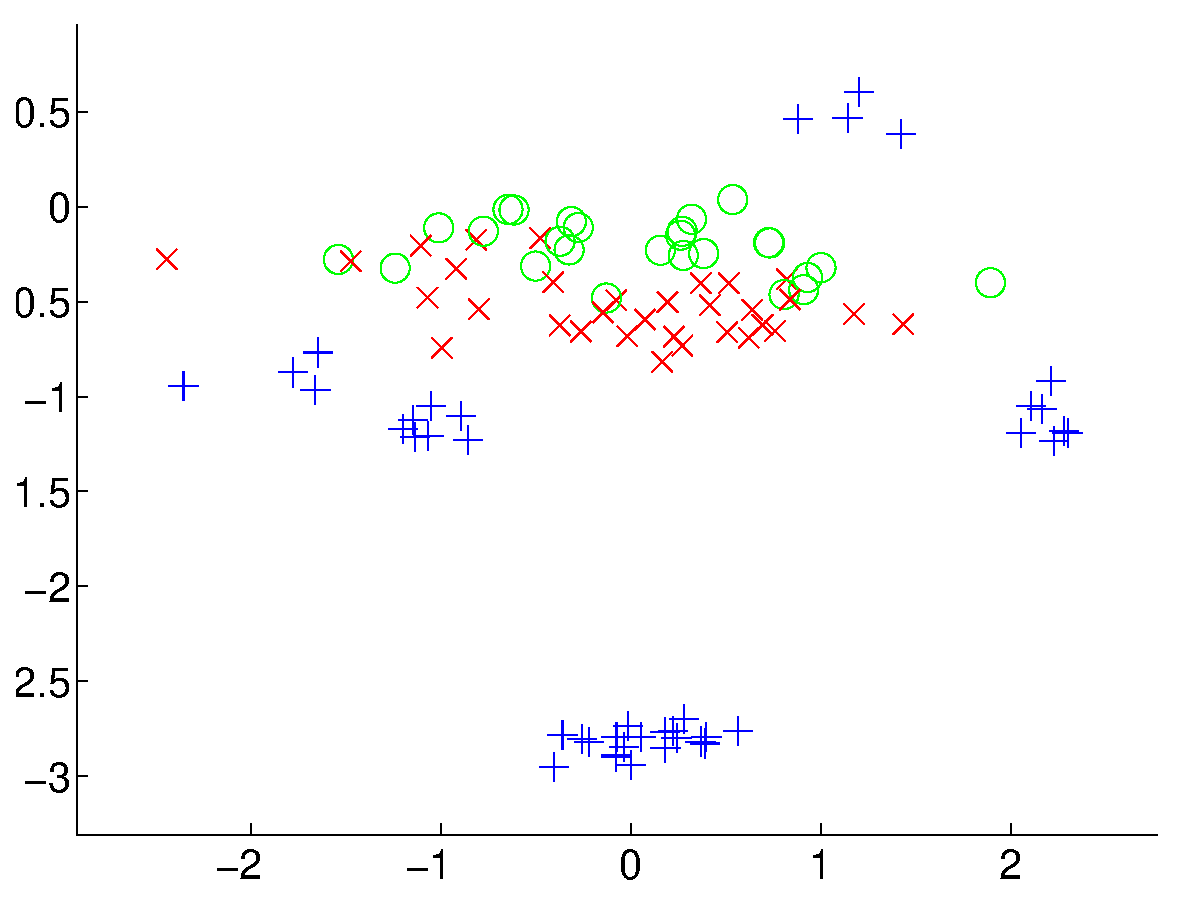
\includegraphics[width=0.42\textwidth,keepaspectratio]{diagrams/pcaOil100}}\hfill{}\subfloat[]{

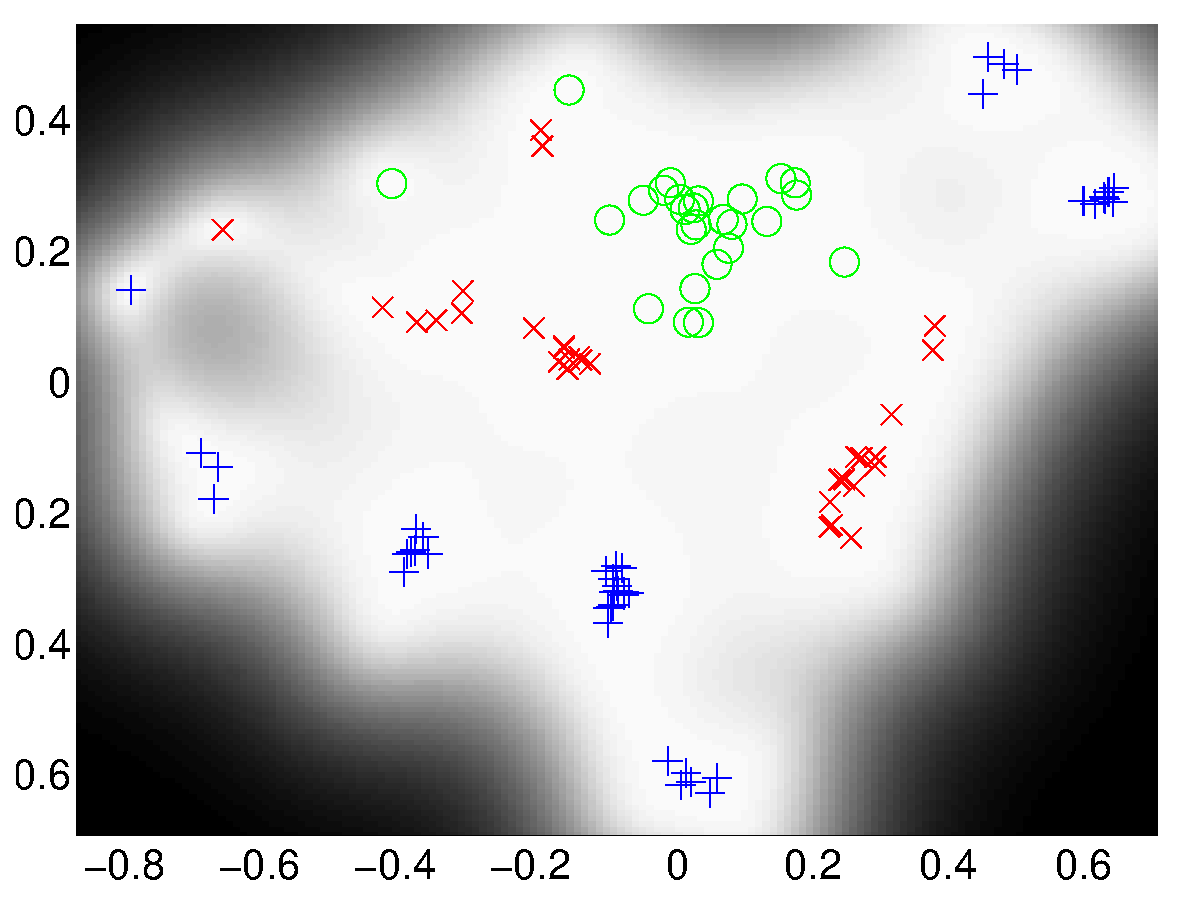
\includegraphics[width=0.42\textwidth,keepaspectratio]{diagrams/gplvmOil100}}\\
\subfloat[]{

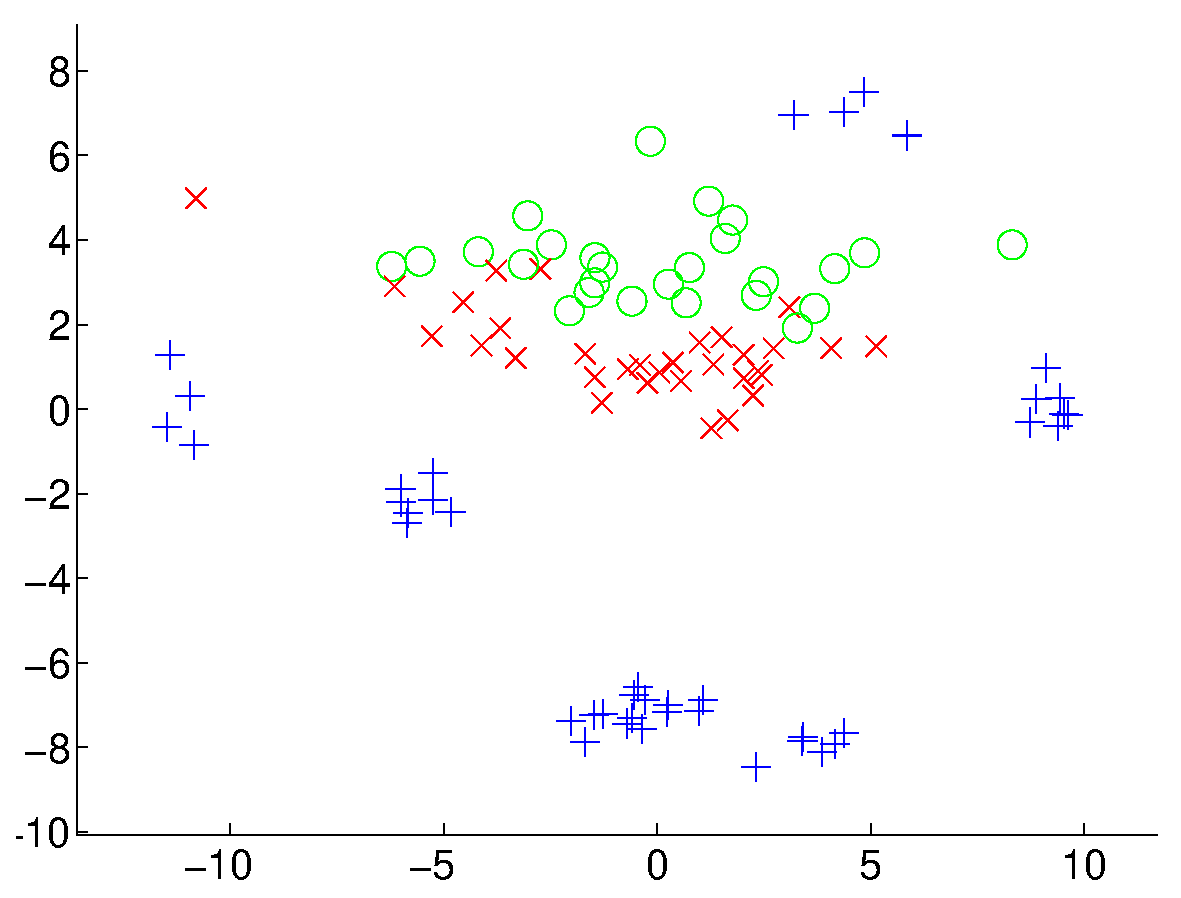
\includegraphics[width=0.42\textwidth,keepaspectratio]{diagrams/nonmetricMdsOil100}}\hfill{}\subfloat[]{

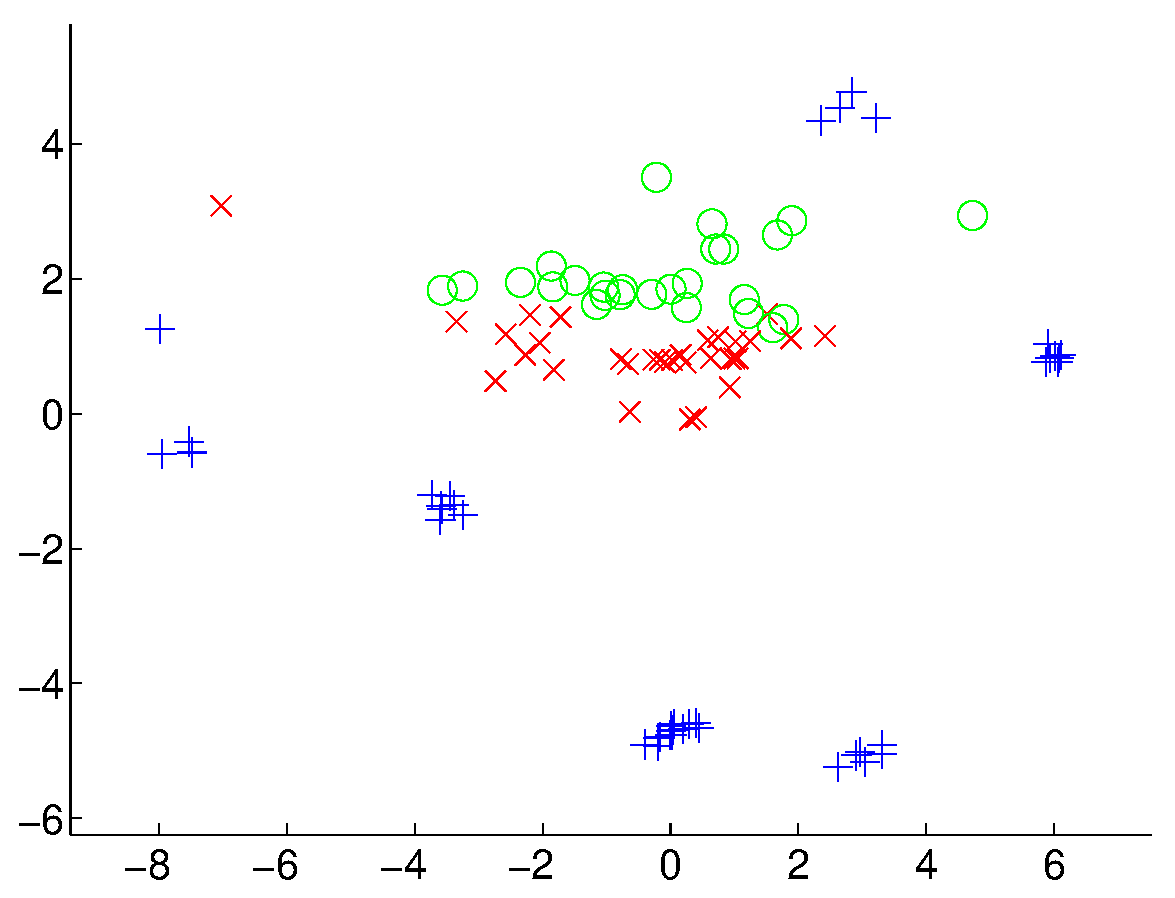
\includegraphics[width=0.42\textwidth,keepaspectratio]{diagrams/sammonOil100}}\\
\subfloat[]{

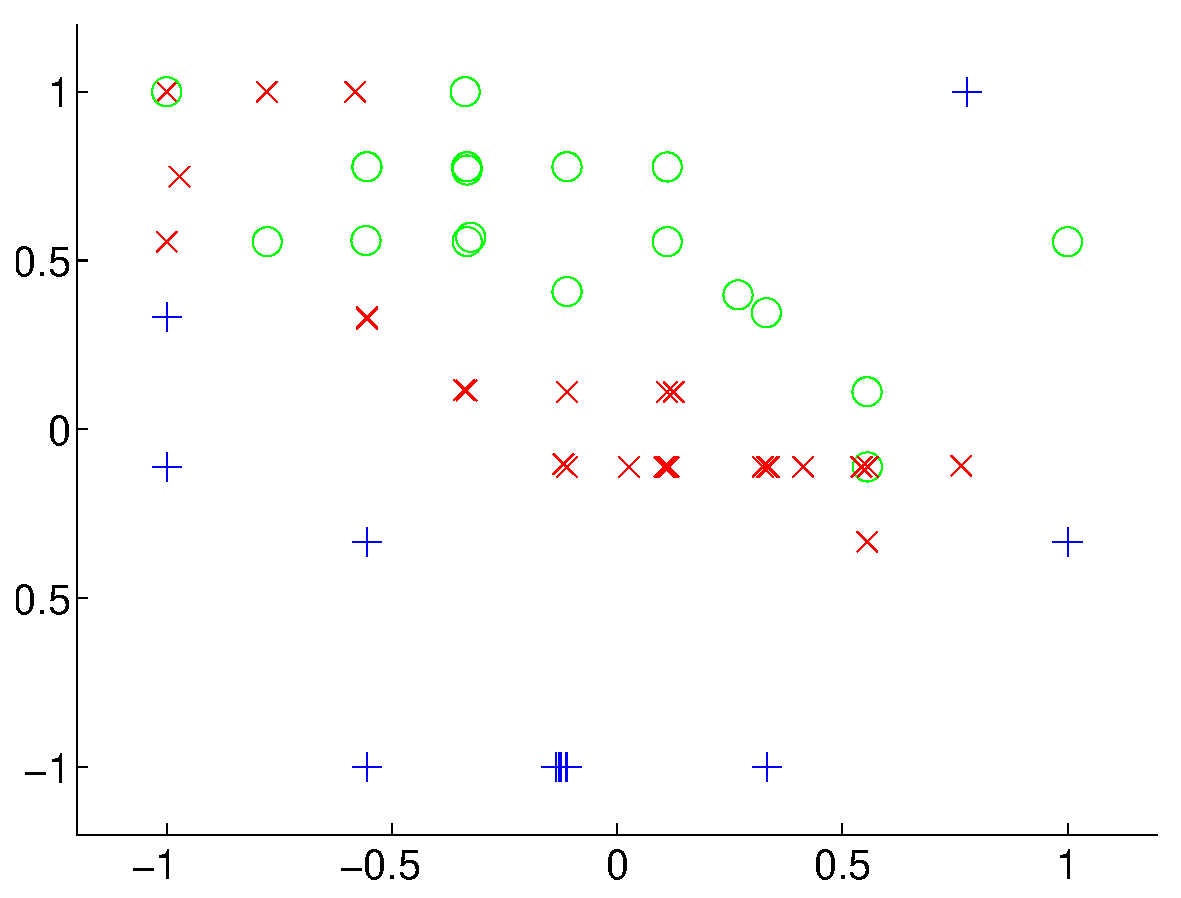
\includegraphics[width=0.42\textwidth,keepaspectratio]{diagrams/gtmOil100}}\hfill{}\subfloat[]{

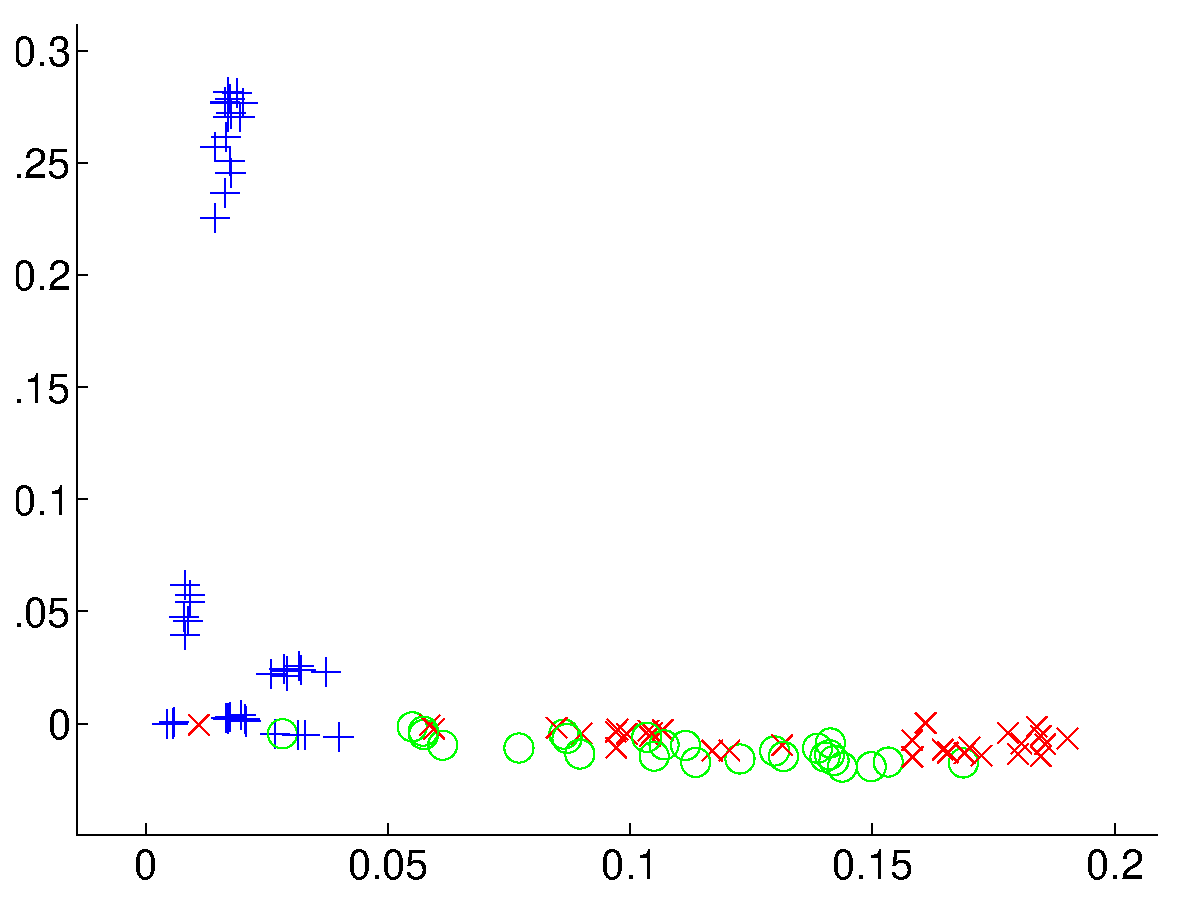
\includegraphics[width=0.42\textwidth,keepaspectratio]{diagrams/kpcaOil100}}\\
\par\end{centering}
\caption{Visualisation of the Oil data with (a) PCA (a linear GP-LVM) and (b)
A GP-LVM which uses an RBF kernel, (c) Non-metric MDS using Kruskal's
stress, (d) M `Sammon Mapping', (e) GTM and (f) kernel PCA. Red crosses,
green circles and blue plus signs represent stratified, annular and
homogeneous flows respectively. The greyscales in plot (b) indicate
the precision with which the manifold is expressed in data-space for
that latent point. \label{cap:oilVisualisation100}}
\end{figure}

The likelihood for the RBF kernel was optimised using scaled conjugate
gradient (see \url{http://www.dcs.shef.ac.uk/~neil/gplvmcpp/} for
the C++ code used).

In Figure~\ref{cap:oilVisualisation100}(c) we show the result of
non-metric MDS using the stress criterion of \citet{Kruskal:mds64}.
Figure~\ref{cap:oilVisualisation100}(d) shows the result from the
`Sammon mapping' \citep{Sammon:nonlinear69}. To objectively evaluate
the quality of the visualisations we classified each data point according
to the class of its nearest neighbour in the two dimensional latent-space
supplied by each method. The errors made by such a classification
are given in Table~\ref{cap:oil100NNErrors}. For the GTM and kernel
PCA some selection of parameters is required. For GTM we varied the
size of the latent grid between $3\times3$ and $15\times15$, and
the number of hidden nodes in the RBF network was varied between 4
and 36. The best result was obtained for a $10\times10$ latent grid
with 25 nodes in the RBF network, it is shown in Figure~\ref{cap:oilVisualisation100}(e).
Note the characteristic gridding effect in the GTM's visualisation
which arises from the layout of the latent points. For kernel PCA
we used the RBF kernel and varied the kernel width between 0.01 and
100. The best result was obtained for a kernel width of 0.75, the
associated visualisation is shown in Figure~\ref{cap:oilVisualisation100}(f).

\begin{table}
\begin{centering}
\begin{tabular}{|c||c|c|c|c|c|c|}
\hline 
Method & PCA & GP-LVM & Non-metric MDS & Metric MDS & GTM{*} & kernel PCA{*}\\ 
\hline 
Errors & 20 & 4 & 13 & 6 & 7 & 13\\ 
\hline 
\end{tabular}
\par\end{centering}
\caption{Errors made by the different methods when using the latent-space for
nearest neighbour classification in the latent space. Both the GTM
and kernel PCA are given asterisks as the result shown is the best
obtained for each method from a range of different parameterisations.\label{cap:oil100NNErrors}}
\end{table}
The gradient based optimisation of the RBF based GP-LVM's latent-space
shows results which are clearly superior (in terms of separation between
the different flow phases) to those achieved by the linear PCA model.
The GP-LVM approach leads to a number of errors that is the smallest
of all the approaches used. Additionally the use of a Gaussian process
to perform our `mapping' means that we can express uncertainty about
the positions of the points in the \emph{data} space. For our formulation
of the GP-LVM the level of uncertainty is shared across all $D$ dimensions
and thus may be visualised in the latent-space. 

\subsubsection{Visualising the Uncertainty\label{subsec:visualisingUncertainty}}

Recall that the likelihood (\ref{eq:gplvmLikelihood}) is a product
of $D$ separate Gaussian processes. In all that has followed we have
retained the implicit assumption in PCA that \emph{a priori} each
dimension is identically distributed by assuming that the processes
shared the same covariance/kernel function $\mathbf{K}.$ Sharing
of the covariance function also leads to an \emph{a posteriori} shared
level of uncertainty in each process. While it is possible to use
different covariance functions for each dimension and may be necessary
when each of the data's attributes have different characteristics\footnote{A simple example of this is given by \citet{Grochow:styleik04} with
the `scaled GP-LVM', where a scale parameter is associated with each
dimension of the data.}; the more constrained model implemented here allows us to visualise
the uncertainty in the latent space and will be preferred for our
empirical studies\footnote{The two approaches, constraining each data direction to the same kernel
and allowing each data dimension to have its own kernel are somewhat
analogous to the difference between probabilistic PCA, where each
output data shares a variance, and factor analysis, where each data
dimension maintains its own variance.}. In Figure~\ref{cap:oilVisualisation100}(b) (and subsequently)
the uncertainty is visualised by varying the intensity of the background
pixels. The lighter the pixel the higher the precision of the mapping.

\subsubsection{Computational Complexity}

While the quality of the results seem good, a quick analysis of the
algorithmic complexity shows that each gradient step requires an inverse
of the kernel matrix (see (\ref{eq:likelihoodGradK})), an $O\left(N^{3}\right)$
operation, rendering the algorithm impractical for many data sets
of interest. 

\subsection{Large Data Sets}

The sparse approximation suggested in \citet{Lawrence:gplvm03,Lawrence:pnpca05}
is a sub-set of data approach \citep[pg. 177]{Lawrence:ivm02,Rasmussen:book06}.
Whilst this approach leads to somewhat simple algorithms for optimisation
of the GP-LVM, it suffers from the lack of a convergence criterion
and discards information in the data set. A more promising approach
to sparsification is suggested for Gaussian process regression by
\citet{Snelson:pseudo05} and has recently be placed in a more general
framework by \citet{Quinonero:unifying05}. The application of this
approach in the GP-LVM is available on-line and is the subject of
a forthcoming paper \citep[in preparation]{Lawrence:largescale06}.

In Figure~\ref{cap:gplvmOilVisualise} we present visualisations
of the oil data using a sub-set of data based sparse GP-LVM algorithm
with the RBF kernel. In Figure~\ref{cap:fullOil} we show the data
visualised with the non-sparse GP-LVM algorithm.
\begin{figure}
\begin{centering}
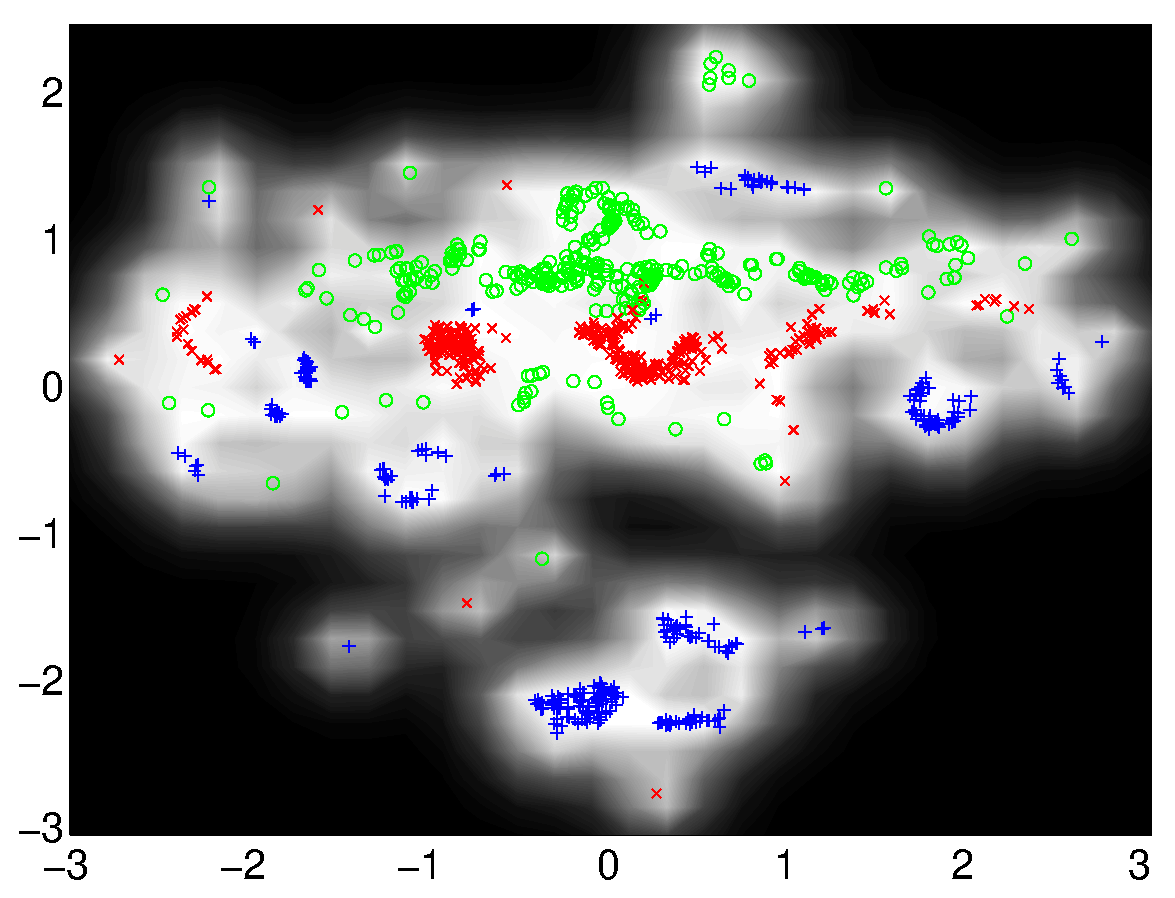
\includegraphics[width=0.75\textwidth,keepaspectratio]{diagrams/trOil1} 
\par\end{centering}
\caption{The full oil flow data set visualised with an RBF based kernel using
sub-set of data approximations.\label{cap:gplvmOilVisualise}}
\end{figure}
\begin{figure}
\begin{centering}
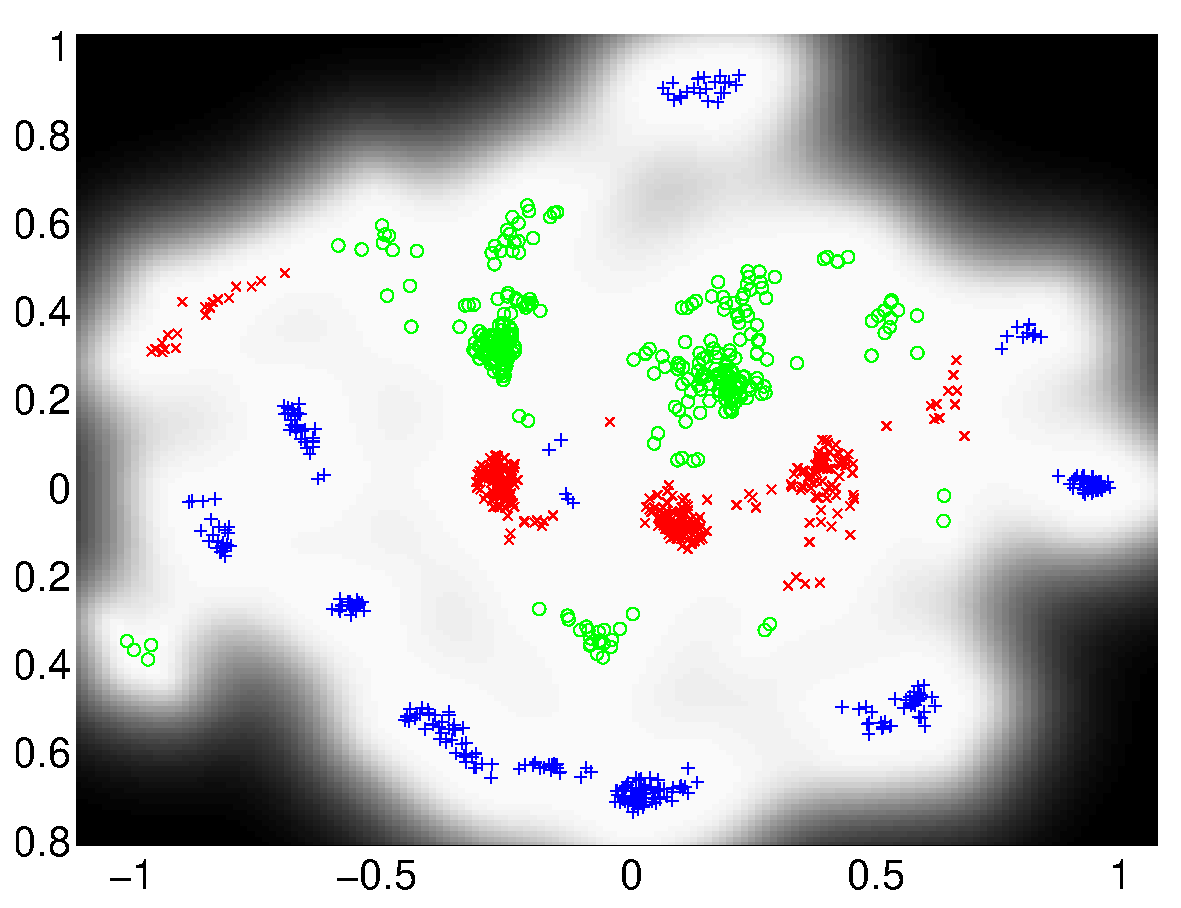
\includegraphics[width=0.75\textwidth,keepaspectratio]{diagrams/fullGplvmOil1000}
\par\end{centering}
\caption{The full GP-LVM algorithm with RBF kernel on the oil flow data (uses
the GPLVMCPP toolbox). \label{cap:fullOil}}
\end{figure}
Again we considered a nearest neighbour classifier in the latent-space
to quantify the quality of the visualisations. 
\begin{table}
\begin{centering}
\begin{tabular}{|c||c|c|c|c|c|}
\hline 
Model & PCA & Sparse GP-LVM (IVM) & GP-LVM (RBF) & GTM & Y\\ 
\hline 
Errors & 162 & 24 & 1 & 11 & 2\\ 
\hline 
\end{tabular}
\par\end{centering}
\caption{Number of errors for nearest neighbour classification in the latent-space
for the full oil data set (1000 points). Far right column contains
result for nearest neighbour in the data space, also presented is
a result for the GTM algorithm.\label{cap:oilClassiificationTable}}
\end{table}
We note that there appears to be a degradation in the quality of the
GP-LVM model associated with the sparsification, in comparision to
the full GP-LVM algorithm and the sub-set of data based sparse GP-LVM
performs worse.

\subsection{Back Constraints}

An interesting characteristic of the GP-LVM is that it provides a
smooth mapping from latent space to the data space. This implies that
points which are close in latent space will be close in data space.
However, it does not imply that points which are close in data space
will be necessarily mapped as close together in latent space. In recent
work \citep[in preparation]{Lawrence:backconstraints06} the use of
back constraints is suggested. Back constraints constrain each latent
points to be a smooth function of its corresponding data point. This
forces points which are close in data space to be close in latent
space. 

\subsubsection{Motion Capture Data}

A neat illustration of the issues that arise when the GP-LVM is used
without back constraints is given by a simple motion capture data
set. The data consists of a subject breaking into a run from standing\footnote{Data made available by the Ohio State University Advanced Computing
Centre for the Arts and Design, available from \url{http://accad.osu.edu/research/mocap/mocap_data.htm},
sequence `Figure Run 1' in unprocessed \texttt{.txt} format.}. There are approximately three full strides in the sequence. The
mean of the data is removed from each frame so in effect the subject
is running `in place'. The data is therefore somewhat periodic in
nature, however the subject changes the angle of the run throughout
the sequence becoming more upright as it proceeds. Our experimental
set up was as follows. For both models a GP-LVM with an RBF kernel
for a covariance function was used. The back constraint was implemented
through an RBF based kernel mapping for which we set $\gamma=1\times10^{-3}$.
Both models were initialised using PCA. For the RBF model this is
straightforward, but for the kernel model this was achieved by setting
the kernel parameters, $\mathbf{A}$, to minimise the squared distance
between the latent positions given by the mapping and those given
by PCA. The latent positions/mapping parameters and the GP covariance
function parameters were then jointly optimised using conjugate gradients.
Scripts for re-implementing these experiments are available on line
in the FGPLVM toolbox.

\begin{figure*}
\begin{centering}
\subfloat[]{

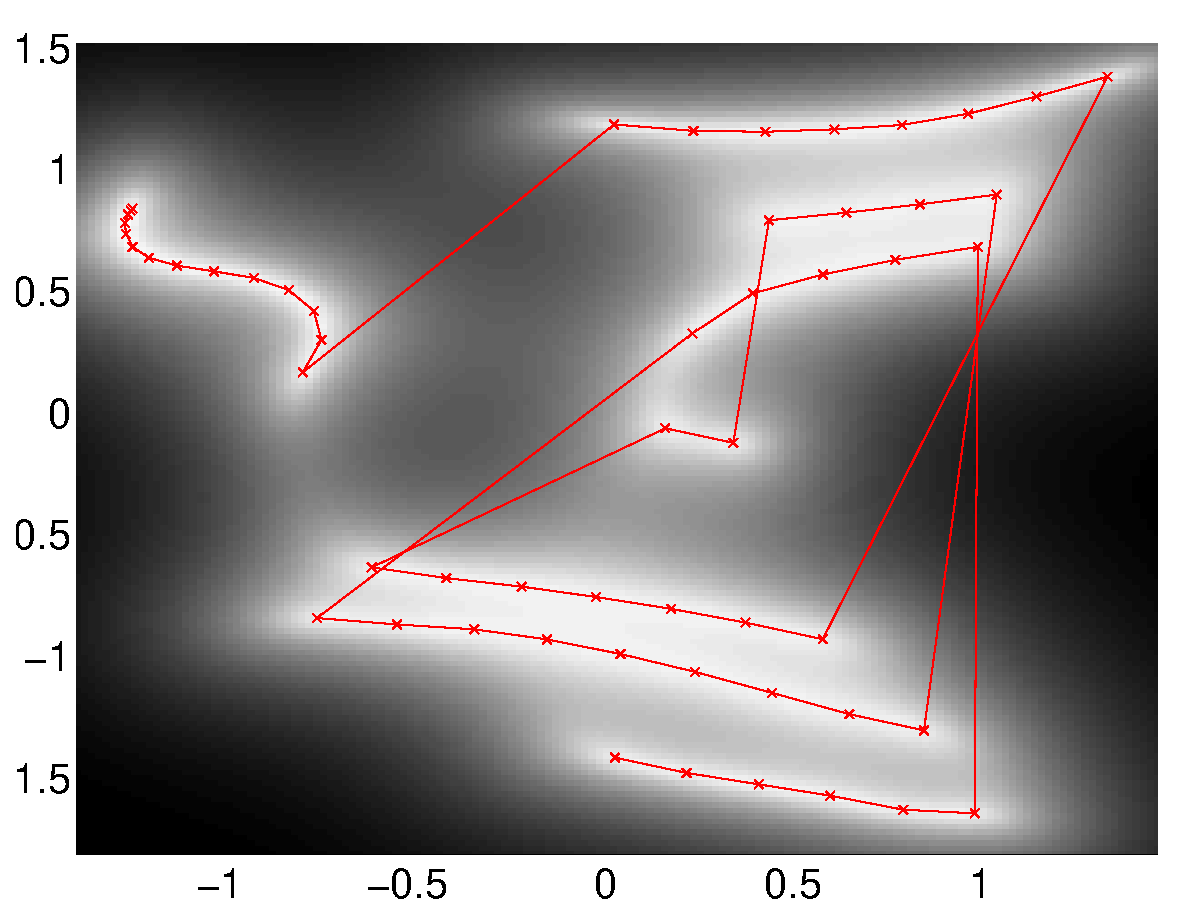
\includegraphics[width=0.45\textwidth]{diagrams/demStick1Connected}}\hfill{}\subfloat[]{

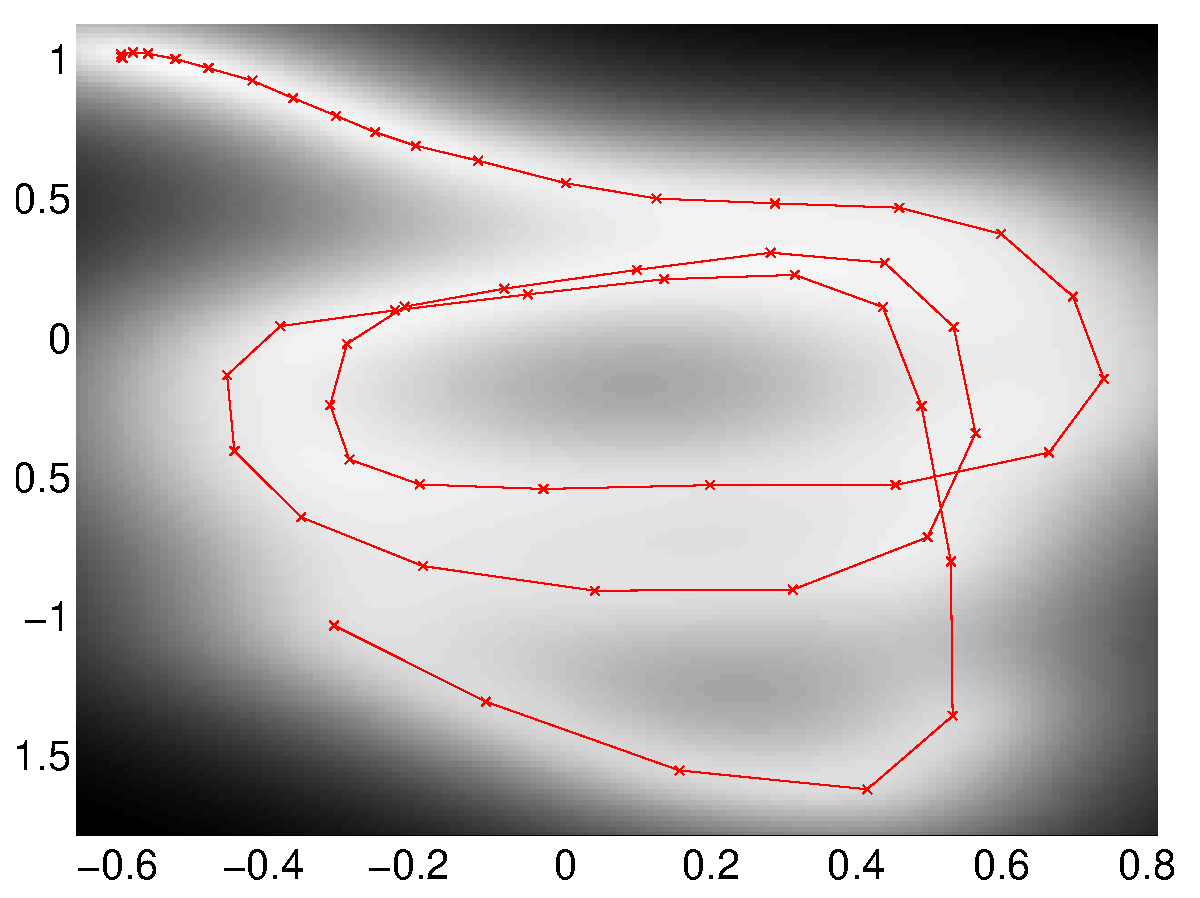
\includegraphics[width=0.45\textwidth]{diagrams/demStick3Connected}}
\par\end{centering}
\caption{Visualisation of the motion capture data. (a) The regular GP-LVM,
log likelihood 1,543 (\texttt{demStick1} in the FGPLVM toolbox) and
(b) the GP-LVM with back constraints (\texttt{demStick3}), log likelihood
1,000. The paths of the sequences through latent space are shown as
solid lines.The back constraint used was an RBF kernel mapping with
$\gamma=1\times10^{-3}$. In both cases the start of the sequence
is towards the top left and the end is towards the bottom centre-left.
The grey scale background image indicates the precision with which
the mapping is expressed.\label{cap:stickManRun}}
\end{figure*}

The results from visualisation using the GP-LVM both in unconstrained
and back constrained forms are shown in Figure~\ref{cap:stickManRun}.
The data is temporal in nature (although the GP-LVM is not taking
advantage of this fact) and we have connected points in the plots
that are neighbours in time. In Figure~\ref{cap:stickManRun}(a)
the sequence does not clearly show the periodic nature of the data.
The likelihood of this model is higher, as we should expect given
that the other model is constrained, however the sequence is split
across several sub-sequences\footnote{Note this is \emph{not} due to overfitting: the model provides a smooth
representation of the data which generalises well across the latent
space.}. To reflect the periodic nature of the sequence it is necessary to
use a circular structure. Such a structure will be of the form of
a squashed spiral which will either have less representational power
in the inner rings (analogous to inner groove distortion in gramophone
records) or will cross over itself in a manner which is not consistent
with the data. The higher likelihood solution turns out to be placing
points far apart which are actually close together. Note that the
problem arises because the latent space is too constrained. Using
a three dimensional latent space alleviates the problem\footnote{A script to run the experiment is available on line (\texttt{demStick4}
in the FGPLVM toolbox).} and we expect a two dimensional latent space which is topologically
cylindrical would also resolve the issue. The back constrained model
shows a squashed spiral structure which reflects the periodic nature
of the data and maintains a representation of the angle of the run.
The changing angle of the run as the sequence proceeds is depicted
in Figure~\ref{cap:stickManRunProjections}.

\begin{figure}
\begin{centering}
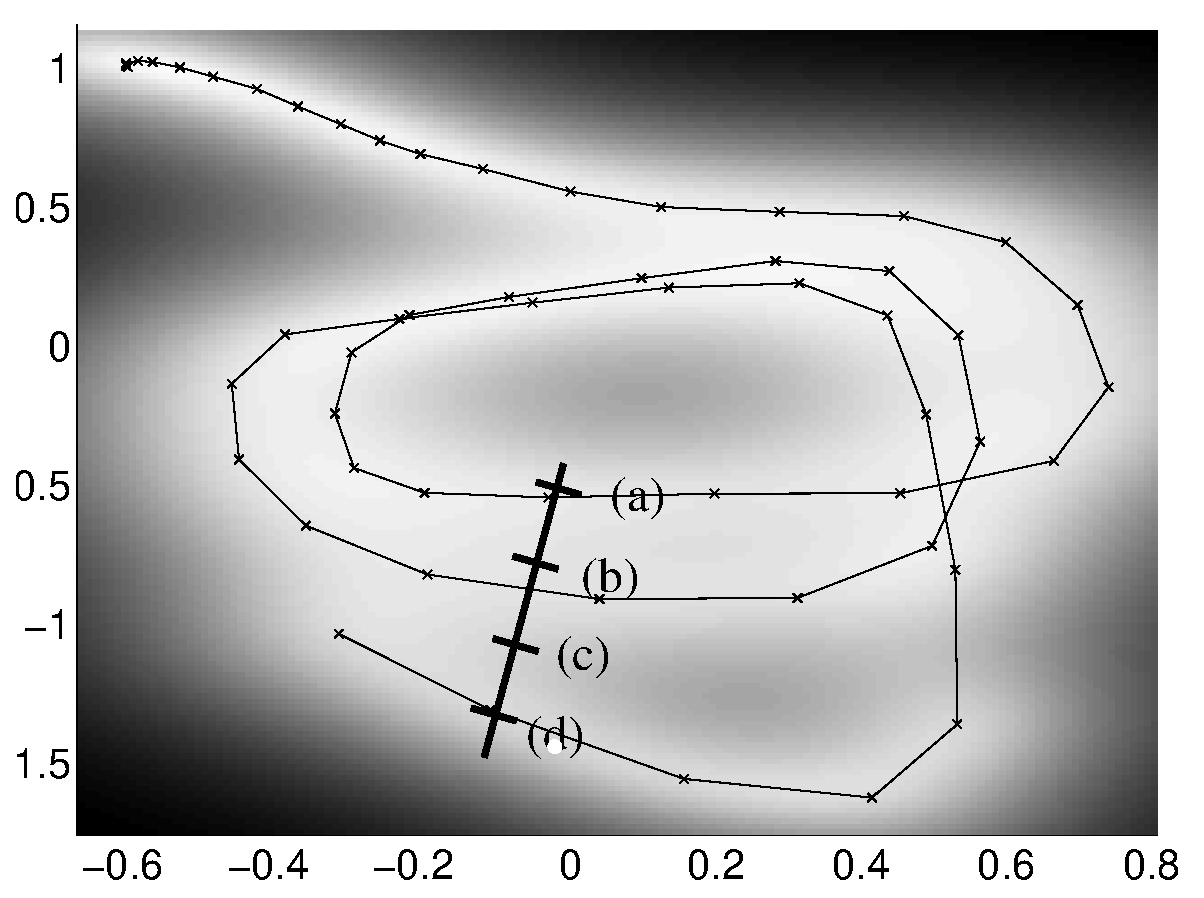
\includegraphics[width=0.8\columnwidth]{diagrams/demStick3AngleLatent}\\
\noindent\begin{minipage}[c][1\totalheight][t]{1\columnwidth}%
\subfloat[]{

\includegraphics[height=1in,keepaspectratio]{diagrams/demStick3Angle1}}\hfill{}\subfloat[]{

\includegraphics[height=1in,keepaspectratio]{diagrams/demStick3Angle2}}\hfill{} \subfloat[]{

\includegraphics[height=1in,keepaspectratio]{diagrams/demStick3Angle3}}\hfill{} \subfloat[]{

\includegraphics[height=1in,keepaspectratio]{diagrams/demStick3Angle4}}%
\end{minipage}
\par\end{centering}
\caption{Projection into data space from four points in the latent space. Note
how the position in the cycle is the same but the inclination of the
runner differs becoming more upright as the sequence proceeds.\label{cap:stickManRunProjections}}
\end{figure}


\subsubsection{Vowel Data}

As a further example we considered a single speaker vowel data set.
The data consists of the cepstral coefficients and deltas of ten different
vowel phonemes and is acquired as part of a vocal joystick system
\citet{Bilmes:vocal06}. A particular characteristic of this data
set is that PCA, which is used as the initalisation when the back
constraints aren't used, fails to separate the data at all. As a result
the non-back constrained model tends to fragment the different vowels.
The results with the back constrianed model tend to keep like vowels
closer together (Figure~\ref{cap:vowelsBack}).

\begin{figure*}
\begin{centering}
\subfloat[]{

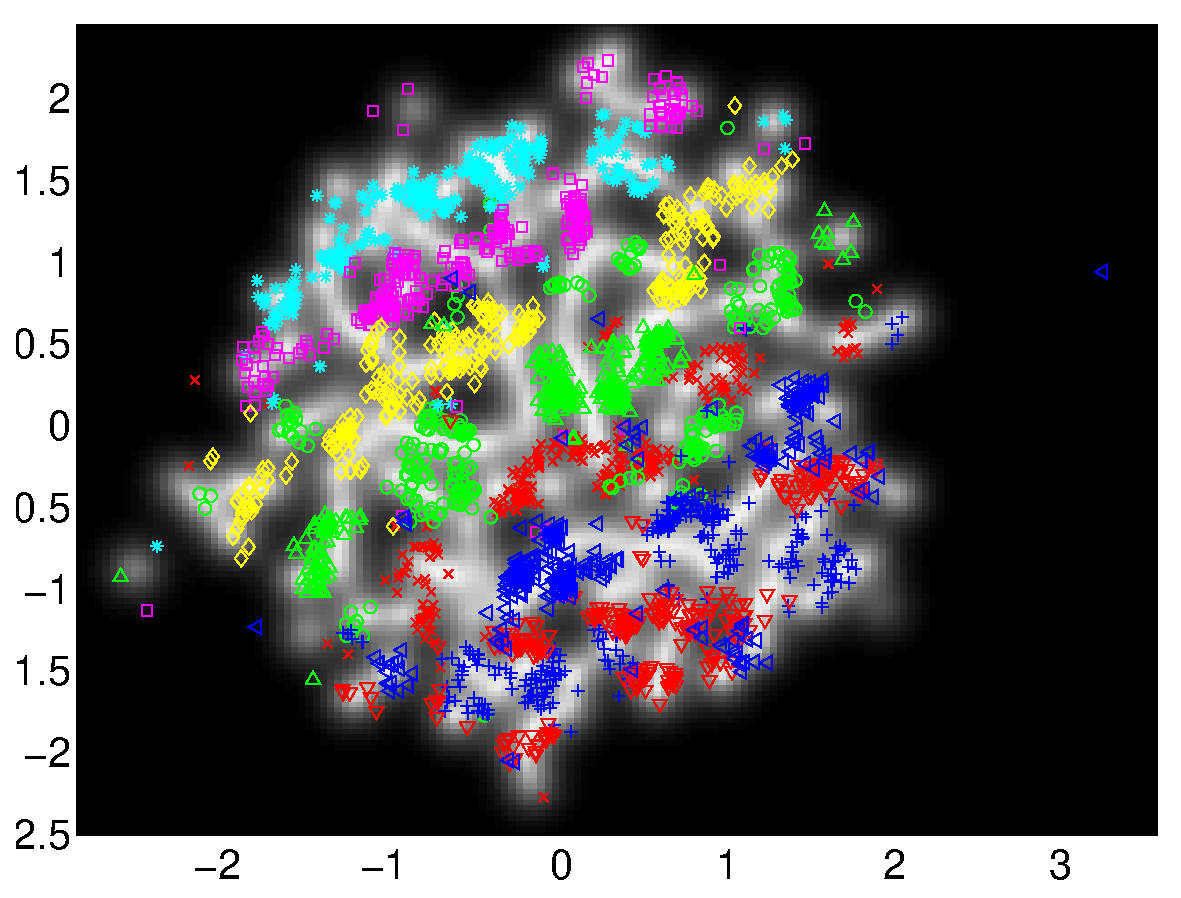
\includegraphics[width=0.8\columnwidth,keepaspectratio]{diagrams/demVowels2}}\\
\subfloat[]{

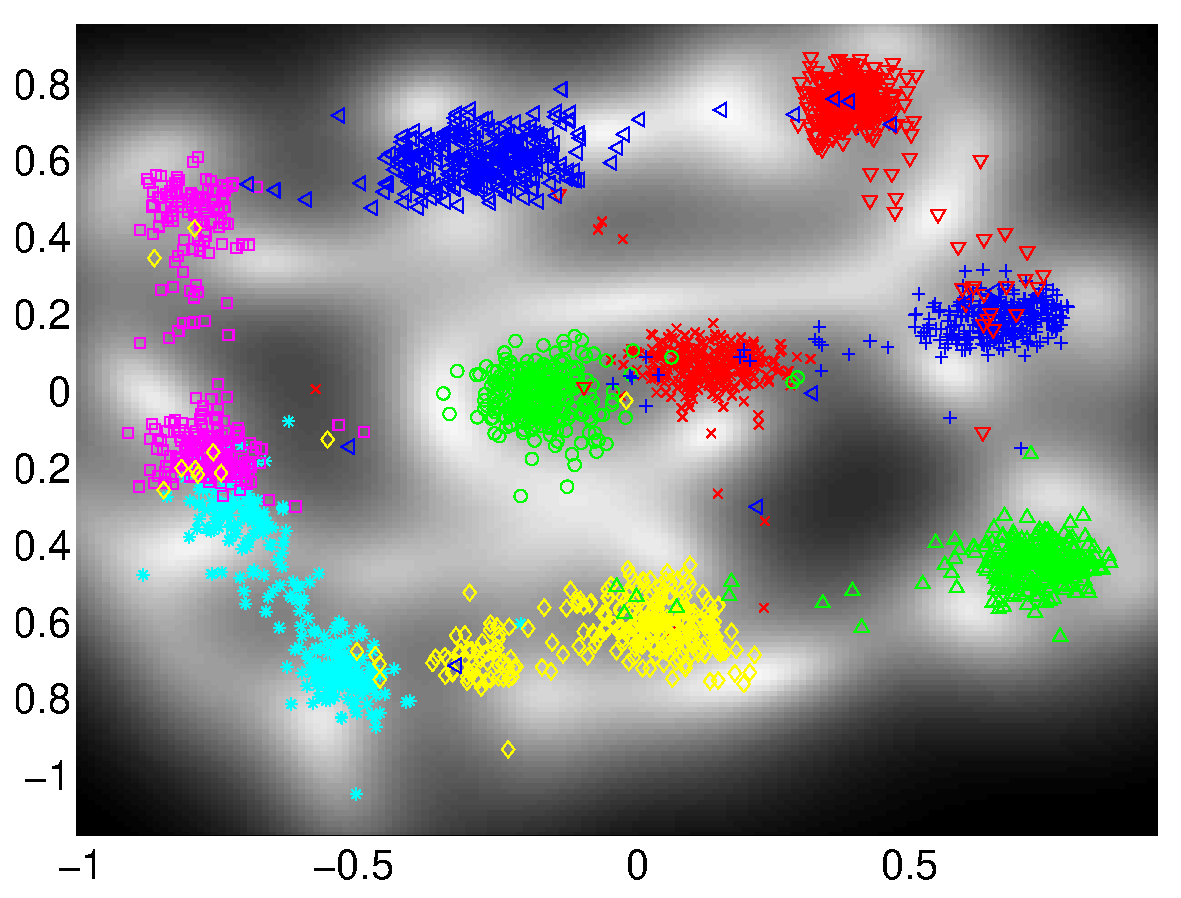
\includegraphics[width=0.8\columnwidth,keepaspectratio]{diagrams/demVowels3}}
\par\end{centering}
\caption{Visualisation of the vowel data (a) without back constraints and (b)
with back constraints. The different vowels are shown as follows:
\emph{/a/} red cross \emph{/ae/} green circle \emph{/ao/} blue plus
\emph{/e/} cyan asterix \emph{/i/} magenta square \emph{/ibar/} yellow
diamond \emph{/o/} red down triangle \emph{/schwa/} green up triangle
and \emph{/u/} blue left triangle (\texttt{\small{}demVowels2} and
\texttt{\small{}demVowels3} in the FGPLVM toolbox).\label{cap:vowelsBack}}
\end{figure*}

\subsection{GP-LVM with Dynamics}

Recently \citet{Wang:gpdm05} described an approach to applying dynamics
to the GP-LVM. To see how this is done, we assume the data is presented
in temporal order (\emph{i.e.}~$\mathbf{y}_{1}$ is the first data
point in the series and $\mathbf{y}_{N}$ is the last). The obvious
route to augmenting the model with dynamics is to place a Markov chain
distribution over the latent space by defining $p\left(\mathbf{x}_{n}|\mathbf{x}_{n-1}\right)$,
which gives a prior distribution $p\left(\mathbf{X}\right)=p\left(\mathbf{x}_{1}\right)\prod_{n=2}^{N}p\left(\mathbf{x}_{n}|\mathbf{x}_{n-1}\right)$.
Of course, combining this prior with $p\left(\mathbf{Y|X}\right)$
to obtain the marginal likelihood $p\left(\mathbf{Y}\right)$ is in
general not tractable. However, it is straightforward to obtain maximum
\emph{a posteriori} (MAP) estimates of the solution. Instead of a
simple Markov chain, \citet{Wang:gpdm05} suggest a Gaussian process
to relate $\mathbf{x}_{n}$ to $\mathbf{x}_{n-1}$. If this GP predicts,
at each time step, the change in position for the next time step,
the joint likelihood over the latent variables and $\mathbf{Y}$ is
given by
\begin{eqnarray}
p\left(\mathbf{Y},\mathbf{X}\right) & = & -\frac{DN}{2}\log2\pi-\frac{D}{2}\log\left|\mathbf{K}\right|-\frac{1}{2}\textrm{tr}\left(\mathbf{K}^{-1}\mathbf{Y}\mathbf{Y}^{\textrm{T}}\right)\nonumber \\
 &  & -\frac{qN}{2}\log2\pi-\frac{q}{2}\log\left|\mathbf{K}_{x}\right|-\frac{1}{2}\textrm{tr}\left(\mathbf{K}_{x}^{-1}\left(\hat{\mathbf{X}}-\mathbf{\tilde{\mathbf{X}}}\right)\left(\hat{\mathbf{X}}-\mathbf{\tilde{\mathbf{X}}}\right)^{\textrm{T}}\right),\label{eq:likelihoodWithDynamics}
\end{eqnarray}
where $\mathbf{\hat{X}}=\left[\mathbf{x}_{2}\dots\mathbf{x}_{N}\right]^{\textrm{T}}$
and $\tilde{\mathbf{X}}=\left[\mathbf{x}_{1}\dots\mathbf{x}_{N-1}\right]^{\textrm{T}}$
the kernel $\mathbf{K}_{x}$ is that associated with the dynamics
Gaussian process and is constructed on the matrix $\tilde{\mathbf{X}}$. 

\subsubsection{Sampling from Dynamics}

Consider a dynamics Gaussian process based on an RBF kernel and a
white noise term,
\[
k\left(\mathbf{x}_{n},\mathbf{x}_{m}\right)=\alpha_{\textrm{rbf}}^{\prime}\exp\left(-\frac{\gamma^{\prime}}{2}\left(\mathbf{x}_{n}-\mathbf{x}_{m}\right)^{\textrm{T}}\left(\mathbf{x}_{n}-\mathbf{x}_{m}\right)\right)+\beta^{\prime-1}\delta_{nm},
\]
where $\delta_{nm}$ is the Kronecker delta function. Rather than
learning the parameters of the dynamics model we suggest an alternative
approach of selecting the dynamics model parameters by hand. Such
an approach may seem unwieldy, but there are only three parameters
in the covariance function, each of which has a clear interpretation.
The signal variance is given by $\alpha_{\textrm{rbf}}^{\prime}$
and the noise variance by $\beta^{\prime-1}$, thus the signal to
noise ratio is given by $\sqrt{\alpha_{\textrm{rbf}}^{\prime}\beta^{\prime}}$.
The remaining parameter controls the smoothness of the function, taking
its square root and inverting, $l=\frac{1}{\sqrt{\gamma}}$, gives
a parameter known as the \emph{characteristic length scale.} In each
dimension the mean level of zero up-crossings in a unit interval is
given by $\left(2\pi l\right)^{-1}=\frac{\sqrt{\gamma}}{2\pi}$ \citep{Rasmussen:book06},
this is related to the number of times the dynamics switches direction.
For the example given below we used $\gamma=0.2$ , $\alpha_{\textrm{rbf}}=0.01$
and $\beta^{-1}=1\times10^{-6}$ which is equivalent to a signal to
noise ratio of 100. In Figure~\ref{cap:dynamicsSamples} we show
some examples of two dimensional dynamics fields sampled using parameters
in the neighbourhood of those given above.

\begin{figure}
\begin{centering}
\subfloat[\foreignlanguage{british}{}]{%

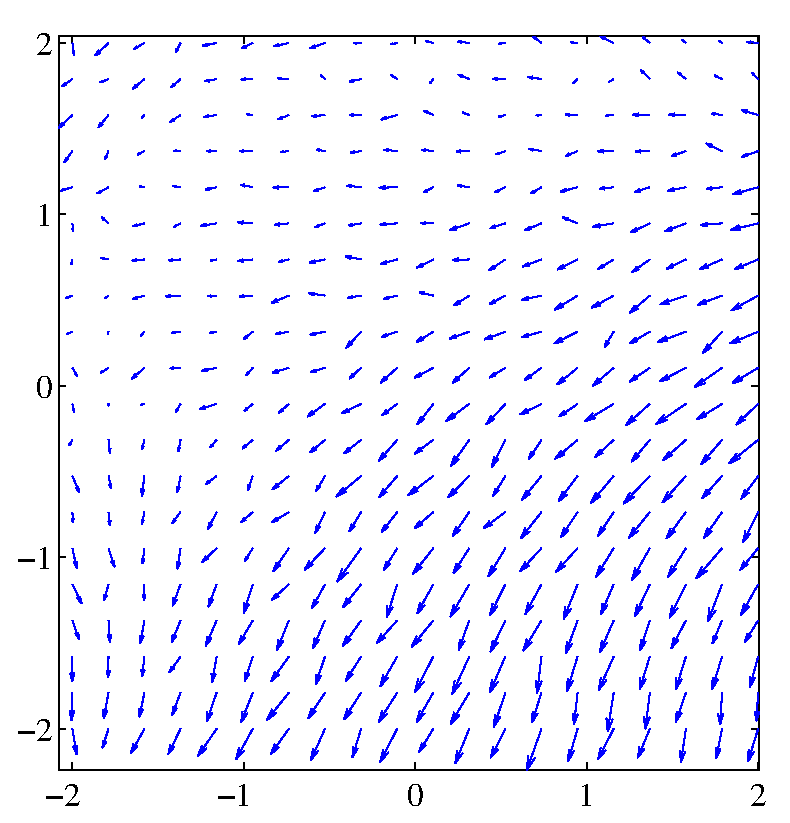
\includegraphics[width=0.3\textwidth]{diagrams/dynSample11}%
}\hfill{}\subfloat[\foreignlanguage{british}{}]{%

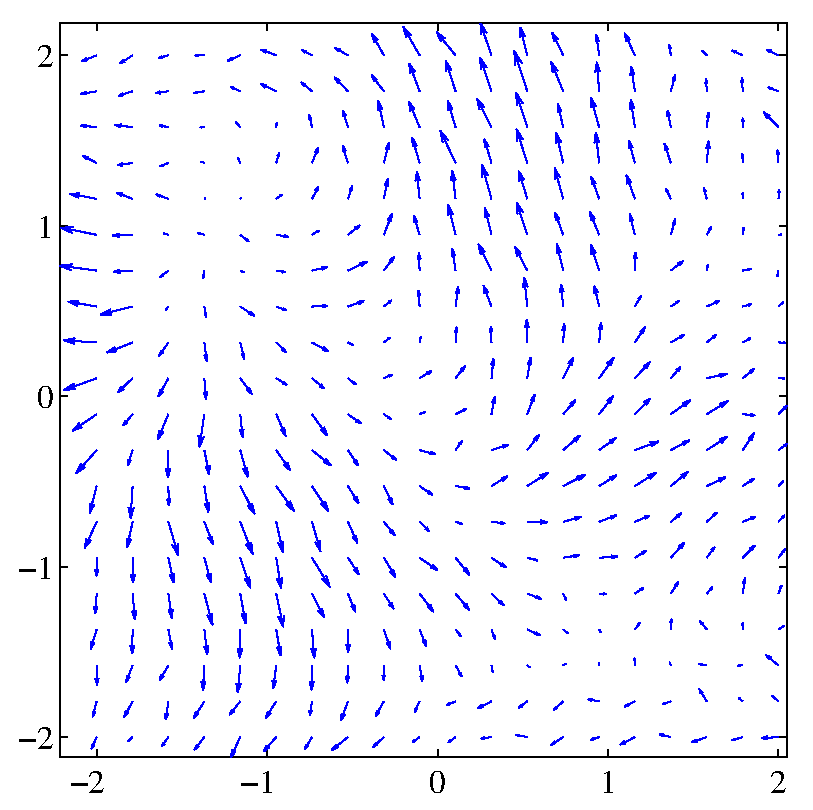
\includegraphics[width=0.3\textwidth]{diagrams/dynSample21}%
}\hfill{}\subfloat[\foreignlanguage{british}{}]{%

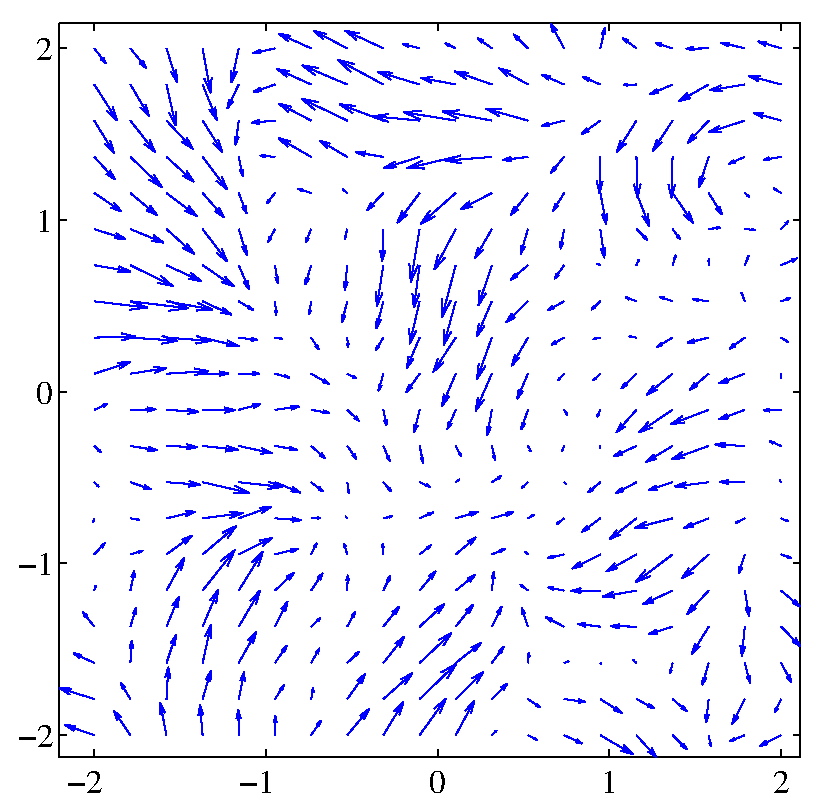
\includegraphics[width=0.3\textwidth]{diagrams/dynSample31}%
}\\
\subfloat[\foreignlanguage{british}{}]{%

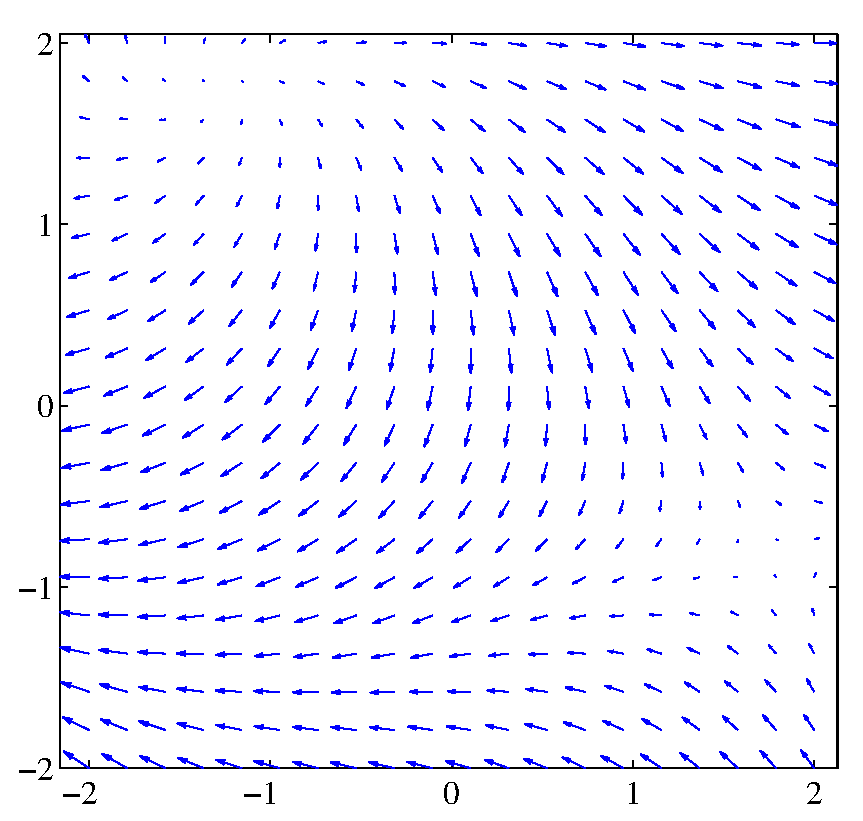
\includegraphics[width=0.3\textwidth]{diagrams/dynSample12}%
}\hfill{}\subfloat[\foreignlanguage{british}{}]{%

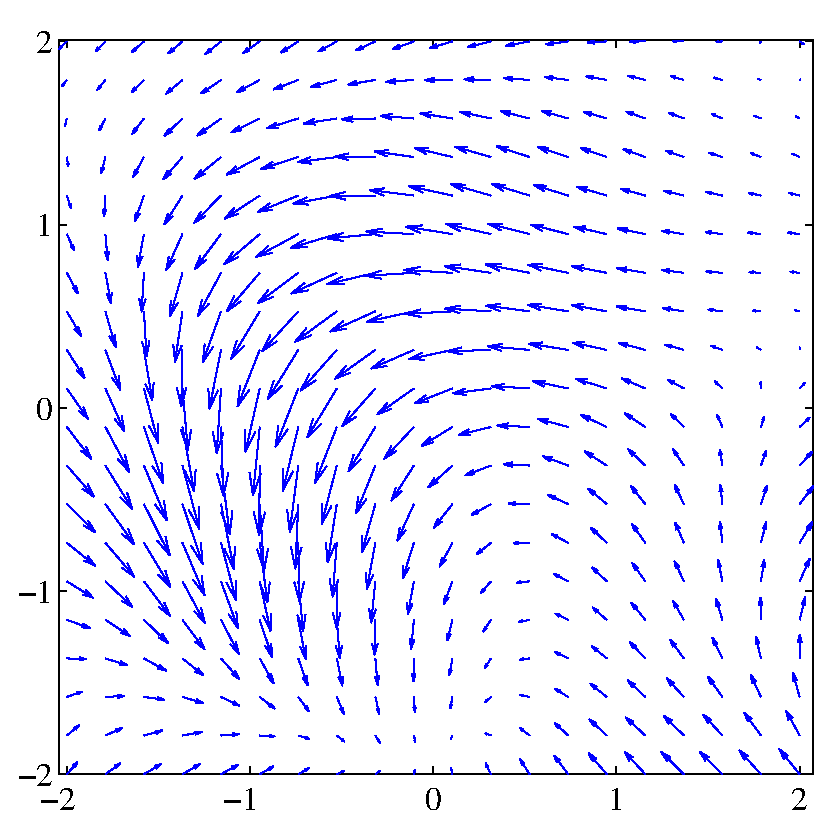
\includegraphics[width=0.3\textwidth]{diagrams/dynSample22}%
}\hfill{}\subfloat[\foreignlanguage{british}{}]{%

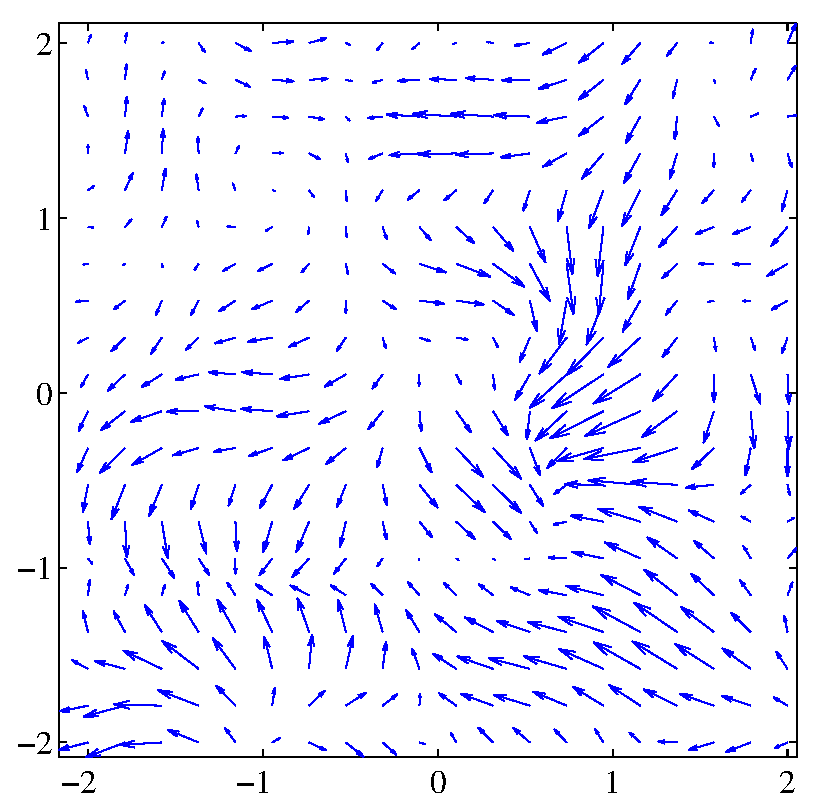
\includegraphics[width=0.3\textwidth]{diagrams/dynSample32}%
}
\par\end{centering}
%
\caption{\foreignlanguage{english}{Samples from the prior over the latent space dynamics. One sample
from each parameterisation is shown. The top row of plots has a signal
to noise ratio of 5 and the bottom row is 100. Length scales decrease
from left to right, left most column $l=2.24$; middle column $l=1$;
and rightmost column $l=0.447$. More specifically the parameters
used in each plot are (a) $\gamma^{\prime}=0.2$, $\beta^{\prime-1}=4\times10^{-4}$,
(b) $\gamma^{\prime}=1$, $\beta^{\prime}=4\times10^{-4}$, (c) $\gamma^{\prime}=5$,
$\beta^{\prime-1}=4\times10^{-4}$, (d) $\gamma^{\prime}=0.2$, $\beta^{\prime-1}=1\times10^{-6}$,
(e) $\gamma^{\prime}=1$, $\beta^{\prime-1}=1\times10^{-6}$ and (f)
$\gamma^{\prime}=5$, $\beta^{\prime-1}=4\times10^{-6}$ with $\alpha_{\textrm{rbf}}^{\prime}=0.1$
for all plots. The overall scale was set to unity. The parameter settings
used to produce Figure~\ref{cap:demStickManDynamics} are associated
with (d).\label{cap:dynamicsSamples}}}
%
\end{figure}


\subsubsection{Motion Capture Data}

By selecting a sensible dynamics prior in the latent space the motion
capture data again reflects the period nature of the paces (Figure~\ref{cap:demStickManDynamics}).

%
\begin{figure}
\begin{centering}
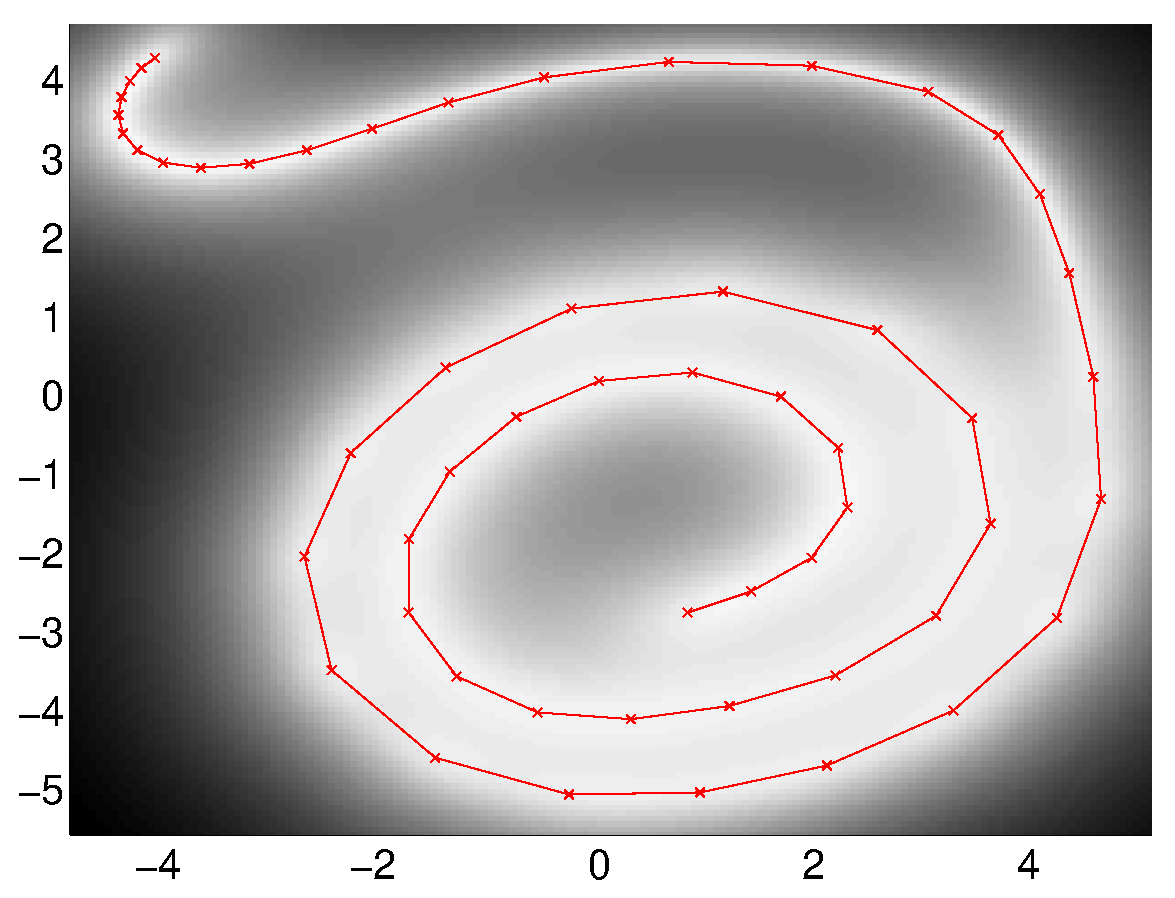
\includegraphics[width=0.45\textwidth]{diagrams/demStick2Connected}
\par\end{centering}
\caption{Visualisation of the motion capture data using the GP-LVM with dynamics
(\texttt{demStick2} in the FGPLVM toolbox) \label{cap:demStickManDynamics}}
\end{figure}


\subsection{Loop Closure in Robotics}

In on-going work with Dieter Fox and Brian Ferris at the University
of Washington we are interested in loop closure for robotic navigation,
included as a final example is a data set of a robot completing a
loop while reading signal strengths from 30 different wireless access
points. To produce a neat track and close the loop it turns out it
is necessary to use dynamics and back constraints as seen in Figure~\ref{cap:wirelessRobot}.
\begin{figure}
\subfloat[]{

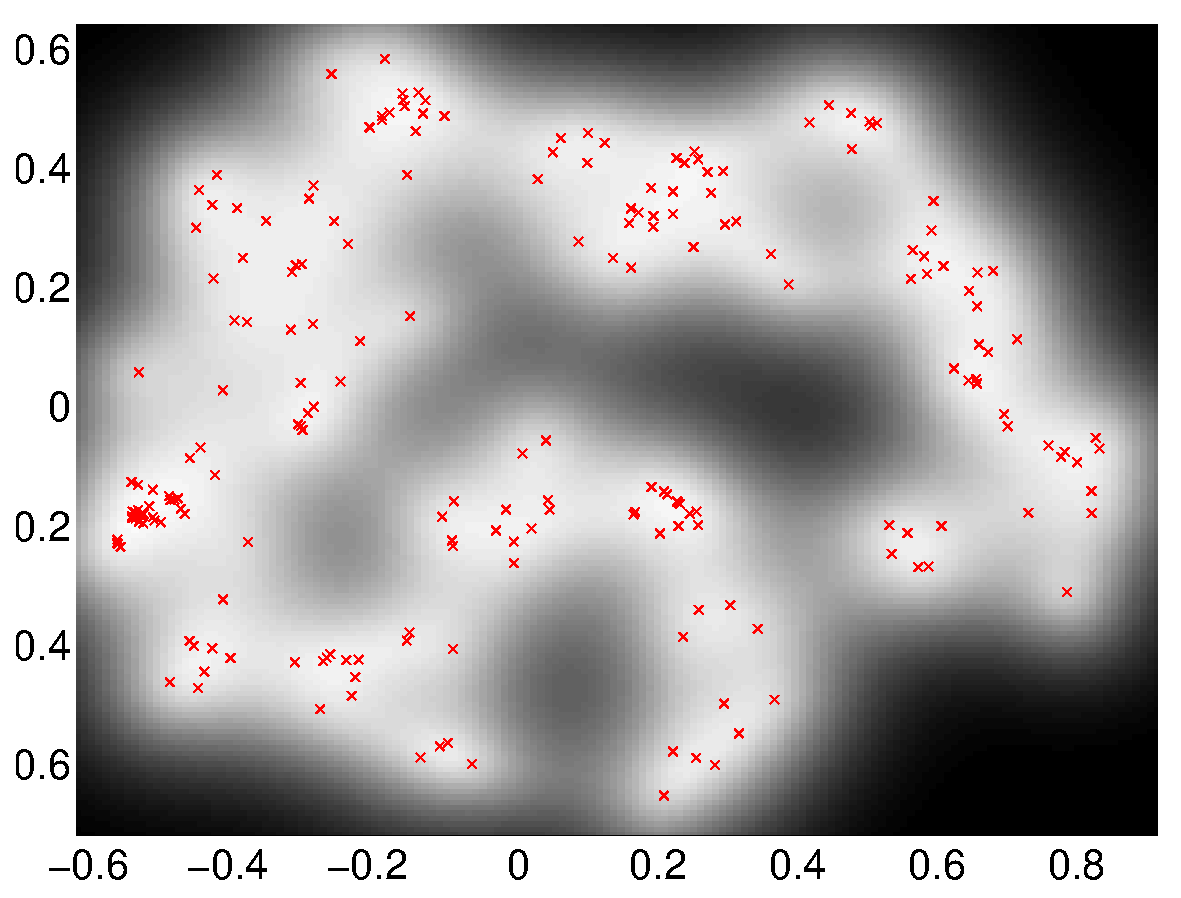
\includegraphics[width=0.45\textwidth]{diagrams/demRobotWireless1}}\hfill{}\subfloat[]{

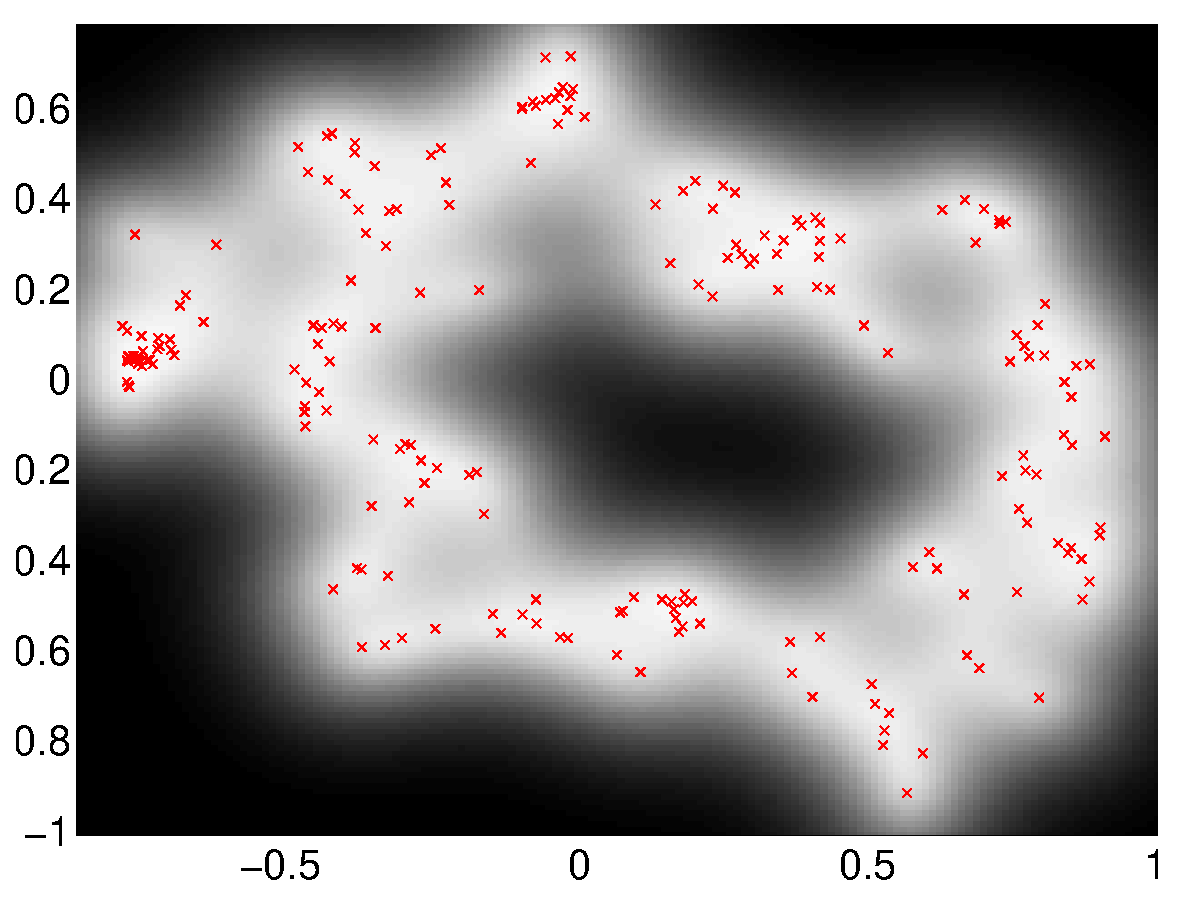
\includegraphics[width=0.45\textwidth]{diagrams/demRobotWireless2}}

\subfloat[]{

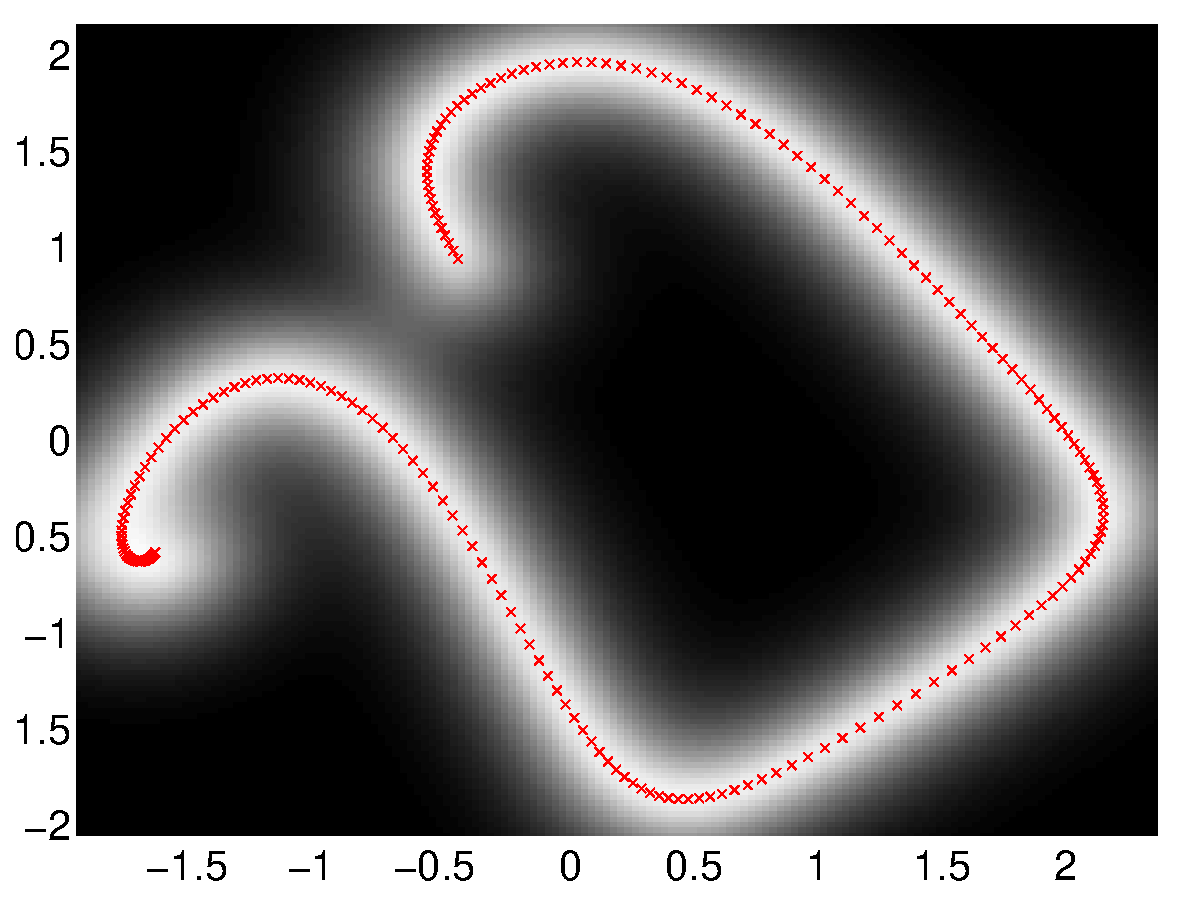
\includegraphics[width=0.45\textwidth]{diagrams/demRobotWireless3}}\hfill{}\subfloat[]{

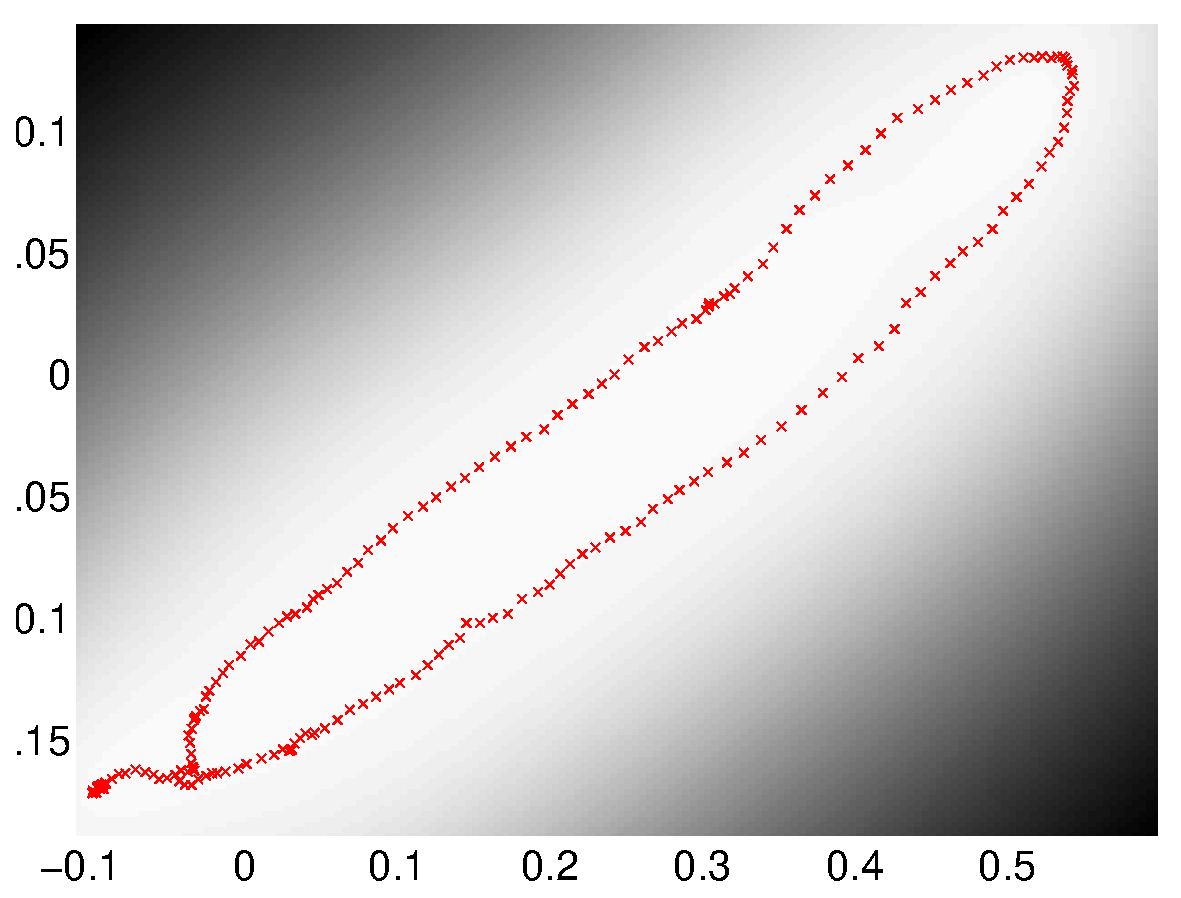
\includegraphics[width=0.45\textwidth]{diagrams/demRobotWireless4}}

\caption{Use of back constraints and dynamics to obtain loop closure in a robot
navigation example. (a) GP-LVM without back constraints or dynamics,
(b) GP-LVM with back constraints, no dynamics, (c) GP-LVM with dynamics,
no back constraints, (d) GP-LVM with back constraints and dynamics.
 These results can be recreated with scripts \texttt{demRobotWireless1}
through \texttt{demRobotWireless4}.\label{cap:wirelessRobot}}
\end{figure}
When the GP-LVM is used without dynamics (Figure~\ref{cap:wirelessRobot}(a)
and (b)) the path in the latent space is noisy. Dynamics forces a
tighter path in latent space (Figure~\ref{cap:wirelessRobot}(c))
but there is no loop closure. Finally by combining back constraints
with dynamics we can obtain loop closure (Figure~\ref{cap:wirelessRobot}(d)).

\section{Conclusion}

This tutorial has aimed to give an overview of the Gaussian process
latent variable model, starting from the perspective of a simple linear
latent variable model, and through the introduction of Gaussian processes,
finishing with a fully probabilistic approach to non-linear dimensionality
reduction. In the results section we showed some simple visualisations
achieved with the algorithm and gave an overview of some of the extensions
to the algorithm. Code for recreating all the results we presented
is available on-line: (\url{http://www.dcs.shef.ac.uk/~neil/gpsoftware.html})
and in many cases we have referred to the specific scripts in captions
of figures. 

\bibliographystyle{abbrvnat}
\bibliography{lawrence,other,zbooks}

\end{document}
